%==============================================================================
% tento soubor pouzijte jako zaklad
% this file should be used as a base for the thesis
% Autoři / Authors: 2008 Michal Bidlo, 2018 Jaroslav Dytrych
% Kontakt pro dotazy a připomínky: dytrych@fit.vutbr.cz
% Contact for questions and comments: dytrych@fit.vutbr.cz
%==============================================================================
% kodovani: UTF-8 (zmena prikazem iconv, recode nebo cstocs)
% encoding: UTF-8 (you can change it by command iconv, recode or cstocs)
%------------------------------------------------------------------------------
% zpracování / processing: make, make pdf, make clean
%==============================================================================
% Soubory, které je nutné upravit: / Files which have to be edited:
%   projekt-20-literatura-bibliography.bib - literatura / bibliography
%   projekt-01-kapitoly-chapters.tex - obsah práce / the thesis content
%   projekt-30-prilohy-appendices.tex - přílohy / appendices
%==============================================================================
\documentclass[cprint]{fitthesis} % bez zadání - pro začátek práce, aby nebyl problém s překladem
%\documentclass[english]{fitthesis} % without assignment - for the work start to avoid compilation problem
%\documentclass[zadani]{fitthesis} % odevzdani do wisu a/nebo tisk s barevnými odkazy - odkazy jsou barevné
%\documentclass[english,zadani]{fitthesis} % for submission to the IS FIT and/or print with color links - links are color
%\documentclass[zadani,print]{fitthesis} % pro černobílý tisk - odkazy jsou černé
%\documentclass[english,zadani,print]{fitthesis} % for the black and white print - links are black
%\documentclass[zadani,cprint]{fitthesis} % pro barevný tisk - odkazy jsou černé, znak VUT barevný
%\documentclass[english,zadani,cprint]{fitthesis} % for the print - links are black, logo is color
% * Je-li práce psaná v anglickém jazyce, je zapotřebí u třídy použít 
%   parametr english následovně:
%   If thesis is written in english, it is necessary to use 
%   parameter english as follows:
%      \documentclass[english]{fitthesis}
% * Je-li práce psaná ve slovenském jazyce, je zapotřebí u třídy použít 
%   parametr slovak následovně:
%   If the work is written in the Slovak language, it is necessary 
%   to use parameter slovak as follows:
%      \documentclass[slovak]{fitthesis}
% * Je-li práce psaná v anglickém jazyce se slovenským abstraktem apod., 
%   je zapotřebí u třídy použít parametry english a enslovak následovně:
%   If the work is written in English with the Slovak abstract, etc., 
%   it is necessary to use parameters english and enslovak as follows:
%      \documentclass[english,enslovak]{fitthesis}

% Základní balíčky jsou dole v souboru šablony fitthesis.cls
% Basic packages are at the bottom of template file fitthesis.cls
% zde můžeme vložit vlastní balíčky / you can place own packages here

\usepackage{tikz}
\usetikzlibrary{arrows,automata, positioning}

\usepackage{pgfplots}
\pgfplotsset{compat=newest}
\usepackage{svg}

\usepackage{xcolor}
\usepackage{bm}
\usepackage{subcaption}

% Kompilace po částech (rychlejší, ale v náhledu nemusí být vše aktuální)
% Compilation piecewise (faster, but not all parts in preview will be up-to-date)
% \usepackage{subfiles}
%\usepackage{subcaption}
%\usepackage{graphicx}

% Nastavení cesty k obrázkům
% Setting of a path to the pictures
%\graphicspath{{obrazky-figures/}{./obrazky-figures/}}
%\graphicspath{{obrazky-figures/}{../obrazky-figures/}}

\renewcommand{\thesection}{\arabic{section}}

%---rm---------------
\renewcommand{\rmdefault}{lmr}%zavede Latin Modern Roman jako rm / set Latin Modern Roman as rm
%---sf---------------
\renewcommand{\sfdefault}{qhv}%zavede TeX Gyre Heros jako sf
%---tt------------
\renewcommand{\ttdefault}{lmtt}% zavede Latin Modern tt jako tt

% vypne funkci šablony, která automaticky nahrazuje uvozovky,
% aby nebyly prováděny nevhodné náhrady v popisech API apod.
% disables function of the template which replaces quotation marks
% to avoid unnecessary replacements in the API descriptions etc.
\csdoublequotesoff

% =======================================================================
% balíček "hyperref" vytváří klikací odkazy v pdf, pokud tedy použijeme pdflatex
% problém je, že balíček hyperref musí být uveden jako poslední, takže nemůže
% být v šabloně
% "hyperref" package create clickable links in pdf if you are using pdflatex.
% Problem is that this package have to be introduced as the last one so it 
% can not be placed in the template file.
\ifWis
\ifx\pdfoutput\undefined % nejedeme pod pdflatexem / we are not using pdflatex
\else
  \usepackage{color}
  \usepackage[unicode,colorlinks,hyperindex,plainpages=false,pdftex]{hyperref}
  \definecolor{hrcolor-ref}{RGB}{223,52,30}
  \definecolor{hrcolor-cite}{HTML}{2F8F00}
  \definecolor{hrcolor-urls}{HTML}{092EAB}
  \hypersetup{
	linkcolor=hrcolor-ref,
	citecolor=hrcolor-cite,
	filecolor=magenta,
	urlcolor=hrcolor-urls
  }
  \def\pdfBorderAttrs{/Border [0 0 0] }  % bez okrajů kolem odkazů / without margins around links
  \pdfcompresslevel=9
\fi
\else % pro tisk budou odkazy, na které se dá klikat, černé / for the print clickable links will be black
\ifx\pdfoutput\undefined % nejedeme pod pdflatexem / we are not using pdflatex
\else
  \usepackage{color}
  \usepackage[unicode,colorlinks,hyperindex,plainpages=false,pdftex,urlcolor=blue,linkcolor=blue,citecolor=black]{hyperref}
  \definecolor{links}{rgb}{0,0,0}
  \definecolor{anchors}{rgb}{0,0,0}
  \def\AnchorColor{anchors}
  \def\LinkColor{links}
  \def\pdfBorderAttrs{/Border [0 0 0] } % bez okrajů kolem odkazů / without margins around links
  \pdfcompresslevel=9
\fi
\fi
% Řešení problému, kdy klikací odkazy na obrázky vedou za obrázek
% This solves the problems with links which leads after the picture
\usepackage[all]{hypcap}

% Informace o práci/projektu / Information about the thesis
%---------------------------------------------------------------------------
\projectinfo{
  %Prace / Thesis
  project={SP},            %typ práce BP/SP/DP/DT/DR  / thesis type (SP = term project)
  year={2020},             % rok odevzdání / year of submission
  date=\today,             % datum odevzdání / submission date
  %Nazev prace / thesis title
  title.cs={Disperze světla},  % název práce v češtině či slovenštině (dle zadání) / thesis title in czech language (according to assignment)
  title.en={Light dispersion}, % název práce v angličtině / thesis title in english
  %title.length={14.5cm}, % nastavení délky bloku s titulkem pro úpravu zalomení řádku (lze definovat zde nebo níže) / setting the length of a block with a thesis title for adjusting a line break (can be defined here or below)
  %Autor / Author
  author.name={Ondřej},   % jméno autora / author name
  author.surname={Pavela},   % příjmení autora / author surname 
  author.title.p={Bc.}, % titul před jménem (nepovinné) / title before the name (optional)
  %author.title.a={Ph.D.}, % titul za jménem (nepovinné) / title after the name (optional)
  %Ustav / Department
  department={UPGM}, % doplňte příslušnou zkratku dle ústavu na zadání: UPSY/UIFS/UITS/UPGM / fill in appropriate abbreviation of the department according to assignment: UPSY/UIFS/UITS/UPGM
  % Školitel / supervisor
  supervisor.name={},   % jméno školitele / supervisor name 
  supervisor.surname={},   % příjmení školitele / supervisor surname
  supervisor.title.p={},   %titul před jménem (nepovinné) / title before the name (optional)
  supervisor.title.a={},    %titul za jménem (nepovinné) / title after the name (optional)
  % Klíčová slova / keywords
  keywords.cs={Disperze světla,
  chromatická disperze, disperzní
  médium, disperzní křivka, fázová rychlost,
  grupová rychlost, anomální disperze, normální
  disperze, index lomu, Snellův zákon,
  spektroskopie}, % klíčová slova v českém či slovenském jazyce / keywords in czech or slovak language
  keywords.en={Sem budou zapsána jednotlivá klíčová slova v anglickém jazyce, oddělená čárkami.}, % klíčová slova v anglickém jazyce / keywords in english
  %keywords.en={Here, individual keywords separated by commas will be written in English.},
  % Abstrakt / Abstract
  abstract.cs={Práce se zabývá fyzikální
  problematikou disperzního jevu se zaměřením
  na jeho projevy v optice. Jsou představeny
  základní fyzikální zákony zodpovědné za
  vznik tohoto jevu spolu s odpovídajícími
  rovnicemi. Důraz je kladen na popis
  disperzních médií, jejich disperzních křivek,
  vysvětlení principu fázové a grupové rychlosti.
  Dále práce rozebírá chromatickou disperzi,
  Snellův zákon a separaci světla na hranolu.
  Součástí práce je demonstrační interaktivní
  program simulující tento jev v paprskové
  optice pomocí algoritmu sledování paprsku.}, % abstrakt v českém či slovenském jazyce / abstract in czech or slovak language
  abstract.en={Do tohoto odstavce bude zapsán výtah (abstrakt) práce v anglickém jazyce.}, % abstrakt v anglickém jazyce / abstract in english
  %abstract.en={An abstract of the work in English will be written in this paragraph.},
  % Prohlášení (u anglicky psané práce anglicky, u slovensky psané práce slovensky) / Declaration (for thesis in english should be in english)
  declaration={Prohlašuji, že jsem tuto bakalářskou práci vypracoval samostatně pod vedením pana X...
Další informace mi poskytli...
Uvedl jsem všechny literární prameny a publikace, ze kterých jsem čerpal.},
  %declaration={I declare that I have prepared this Bachelor´s/Master´s/dissertation thesis independently, under the supervision of ...
% ... provided me with further information.
% I listed all of the literary sources and publications that I have used.},
  % Poděkování (nepovinné, nejlépe v jazyce práce) / Acknowledgement (optional, ideally in the language of the thesis)
  acknowledgment={V této sekci je možno uvést poděkování vedoucímu práce a těm, kteří poskytli odbornou pomoc
(externí zadavatel, konzultant, apod.).},
  %acknowledgment={Here it is possible to express thanks to the supervisor and to the people which provided professional help
%(external submitter, consultant, etc.).},
  % Rozšířený abstrakt (cca 3 normostrany) - lze definovat zde nebo níže / Extended abstract (approximately 3 standard pages) - can be defined here or below
  %extendedabstract={Do tohoto odstavce bude zapsán rozšířený výtah (abstrakt) práce v českém (slovenském) jazyce.},
  %faculty={FIT}, % FIT/FEKT/FSI/FA/FCH/FP/FAST/FAVU/USI/DEF
  faculty.cs={Fakulta informačních technologií}, % Fakulta v češtině - pro využití této položky výše zvolte fakultu DEF / Faculty in Czech - for use of this entry select DEF above
  faculty.en={Faculty of Information Technology}, % Fakulta v angličtině - pro využití této položky výše zvolte fakultu DEF / Faculty in English - for use of this entry select DEF above
  department.cs={Ústav matematiky}, % Ústav v češtině - pro využití této položky výše zvolte ústav DEF nebo jej zakomentujte / Department in Czech - for use of this entry select DEF above or comment it out
  department.en={Institute of Mathematics} % Ústav v angličtině - pro využití této položky výše zvolte ústav DEF nebo jej zakomentujte / Department in English - for use of this entry select DEF above or comment it out
}

% Rozšířený abstrakt (cca 3 normostrany) - lze definovat zde nebo výše / Extended abstract (approximately 3 standard pages) - can be defined here or above
%\extendedabstract{Do tohoto odstavce bude zapsán výtah (abstrakt) práce v českém (slovenském) jazyce.}

% nastavení délky bloku s titulkem pro úpravu zalomení řádku - lze definovat zde nebo výše / setting the length of a block with a thesis title for adjusting a line break - can be defined here or above
%\titlelength{14.5cm}


% řeší první/poslední řádek odstavce na předchozí/následující stránce
% solves first/last row of the paragraph on the previous/next page
\clubpenalty=10000
\widowpenalty=10000

% checklist
\newlist{checklist}{itemize}{1}
\setlist[checklist]{label=$\square$}

\setlength{\parskip}{0pt}

\begin{document}
  % Vysazeni titulnich stran / Typesetting of the title pages
  % ----------------------------------------------
  \maketitle
  % Obsah
  % ----------------------------------------------
  {\hypersetup{hidelinks}\tableofcontents}
  
  % Seznam obrazku a tabulek (pokud prace obsahuje velke mnozstvi obrazku, tak se to hodi)
  % List of figures and list of tables (if the thesis contains a lot of pictures, it is good)
  \ifczech
    \renewcommand\listfigurename{Seznam obrázků}
  \fi
  \ifslovak
    \renewcommand\listfigurename{Zoznam obrázkov}
  \fi
  % \listoffigures
  
  \ifczech
    \renewcommand\listtablename{Seznam tabulek}
  \fi
  \ifslovak
    \renewcommand\listtablename{Zoznam tabuliek}
  \fi
  % \listoftables 

  \ifODSAZ
    \setlength{\parskip}{0.5\bigskipamount}
  \else
    \setlength{\parskip}{0pt}
  \fi

  % vynechani stranky v oboustrannem rezimu
  % Skip the page in the two-sided mode
  \iftwoside
    \cleardoublepage
  \fi

  \clearpage
  % Text prace / Thesis text
  % ----------------------------------------------
  %===============================================================================
% Autoři: Michal Bidlo, Bohuslav Křena, Jaroslav Dytrych, Petr Veigend a Adam Herout 2018

\definecolor{mygreen}{rgb}{0.541,0.886,0.204}

\section{Úvod}
Disperze je všudypřítomný fyzikální jev jehož
dopady jsou pro nás často nežádoucí, ale
existuje i mnoho praktických aplikací, které
naopak tohoto jevu s~výhodou využívají.
Tato práce představuje konkrétně problematiku
disperze světla a přináší základní vhled do
fyzikální teorie za tímto jevem. Jsou zde
představeny
základní fyzikální zákony, kterými se disperze
světla řídí a tak je nutné poznamenat, že se
často jedná o~zjednodušený popis a mnohé
rovnice pouze hrubě aproximují skutečné
jevy. Cílem této práce ovšem nebyl detailní
rozbor tohoto fyzikálního jevu a zájemcům
o~hlubší vhled do této problematiky se tedy
doporučuje vyhledat odbornou literaturu.

\section{Disperze}
Na úvod je nutné poznamenat, že disperze jakožto
fyzikální jev je velmi široký pojem, který se netýká
pouze optiky a separace polychromatického světla
na jednotlivé složky v~důsledku rozdílných indexů lomu
je pouze jedním z~mnoha projevů disperze. Projevy
disperze je tedy možné pozorovat například i
u~mechanického nebo zvukového vlnění a nikoliv pouze
u~elektromagnetického vlnění či viditelného
světla. Tento text se ovšem ze zřejmých důvodů
zabývá pouze disperzí a jejími projevy u~světla.

\subsection{Disperze v~optice}
V~základní podobě se jedná jev, kdy \textit{fázová
rychlost} vlny závisí na její frekvenci, což nastává
pokud se vlna šíří v~takzvaném 
\textit{disperzním prostředí}. Pro jednoduché
monochromatické vlny by se mohlo
zdát, že nám tento jev nezpůsobí příliš mnoho
problémů. Jakmile ovšem začneme uvažovat například
o~přenosu informace pomocí obdélníkových pulzů,
zjistíme, že situace není zdaleka tak jednoduchá.
Dokonalé obdélníkové pulzy se totiž skládají
z~nekonečně mnoha harmonických složek o~různých
frekvencích, jak je možné
ukázat pomocí Fourierovy analýzy. Jev disperze
ovšem není limitován pouze na teoretické úvahy
a lze demonstrovat i na produkovatelných
nedokonalých obdélníkových pulzech, které se
skládají z~konečného počtu harmonických složek.

Efekt disperze u~takového pulzu je znázorněn na
obrázku~\ref{fig:square_wave_disp}, kde
\textit{transceiver} křivka odpovídá výchozí
podobě signálu u~zdroje a \textit{receiver}
křivka odpovídá signálu detekovanému u~přijímače
po průchodu disperzním médiem.
\begin{figure}[htbp]
    \centering
    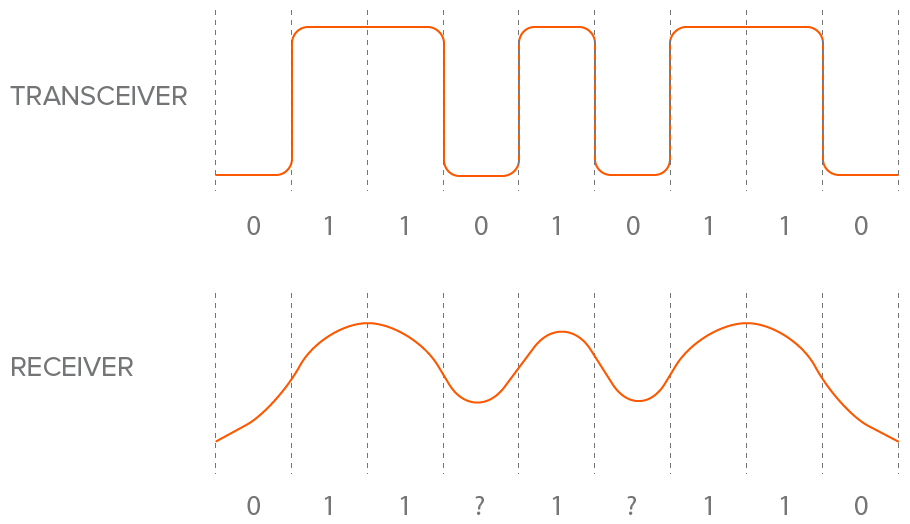
\includegraphics[scale=0.28]{img/BroadeningSignals.png}
    \caption{Znázornění disperzního jevu u~obdélníkových
    pulzů}
    \label{fig:square_wave_disp}
\end{figure}
Zde je možné pozorovat, že na straně přijímače
signál ztratil svůj původní tvar, konkrétně došlo
ke ztrátě vysokofrekvenčních změn v~signálu a
obdélníkové pulzy se rozprostřely v~čase. Důvodem
je právě skutečnost, že se pulzy skládají z~mnoha
harmonických složek o~různých frekvencích, které
médiem putují s~rozdílnými fázovými rychlostmi, což
se projevuje například tak, že složky s~vyššími
frekvencemi mají vyšší fázovou rychlost a
předbíhají tak původní pulz. Naproti tomu
složky s~nižšími frekvencemi mají nižší
fázovou rychlost a opožďují se tedy oproti
původnímu pulzu. Výsledkem je poté degradovaný
signál z~obrázku~\ref{fig:square_wave_disp},
kde došlo k~nežádoucímu rozprostření energie
v~čase. Konkrétní příklad postupné disperze
Gaussova pulzu v~čase je možné pozorovat \href{https://www.acs.psu.edu/drussell/Demos/Dispersion/dispersion.html}{zde}.

Nezbytnou podmínkou disperzního jevu je tedy
průchod disperzním médiem, jehož materiálové
charakteristiky způsobují disperzi.
Materiálovou disperzi můžeme popsat tzv.
\textit{disperzní závislostí}, na základě které
jsme schopni určit, jakou fázovou rychlost
budou mít jednotlivé složky o~různých frekvencích,
viz obrázek~\ref{fig:dispersion_rel}. Disperzní
závislost bude detailněji popsána v~následující
kapitole.
\begin{figure}[htbp]
\centering
\begin{tikzpicture}
\begin{axis}[xmax=5,ymax=5,samples=500,grid=major,
xlabel={k},ylabel={$\omega(k)$}, width=10cm, height=7cm,
minor tick num=1,
grid=major,
axis lines=middle,
enlargelimits={abs=0.5},
ytick={0,1,...,5},
ticklabel style={font=\tiny,fill=white},
legend style={at={(1.5,1)}},
]

\addplot[blue, ultra thick, 
domain=0:4,
label=test,
mark=none,
samples=200,
unbounded coords=jump] {x * sqrt(1 + 0.05 * x^2)};

\addplot[red, ultra thick, 
domain=0:5,
dashed,
mark=none,
samples=200,
unbounded coords=jump] {x};

\addlegendentry{Disperzní médium}
\addlegendentry{Ne-disperzní médium}
\end{axis}
\end{tikzpicture}
\caption{Křivka disperzní závislosti
pro určení fázové rychlosti}
\label{fig:dispersion_rel}
\end{figure}

Často se také
materiálová disperze popisuje disperzní
křivkou, která určuje, jak se mění index
lomu materiálu na základě vlnové délky, viz
obrázek~\ref{fig:dispersion_curves}. Z~obrázku
je patrné, že pro různé materiály jsou křivky
odlišné, přičemž šedá oblast odpovídá viditelné
části spektra.
\begin{figure}[htbp]
    \centering
    \includesvg[scale=0.6]{img/dispersion_curves}
    \caption{Disperzní křivka udávající vztah
    mezi vlnovou délkou a indexem lomu materiálu}
    \label{fig:dispersion_curves}
\end{figure}

Kromě toho existuje i tzv. vlnovodová disperze,
se kterou se nejčastěji setkáme při práci
s~optickými vlákny a která k~celkové disperzi
přispívá nezanedbatelnou částí. Obecně se
vlnovodová disperze může projevit při šíření
vlny libovolným materiálem s~nehomogenní
strukturou, např. fotonickým krystalem, který
se dnes již také využívá v~optických
vláknech~\cite{ing_prace}. Běžně se ovšem
vlnovodová disperze odvíjí od geometrických
charakteristik vlákna, přesněji od poměru
mezi vlnovou délkou světla a poloměrem jádra
vlákna a také od profilu indexu lomu. Dle
citace: \uv{\textit{Tedy i za podmínek nulové
materiálové disperze je skupinové zpoždění
a konstanta šíření každého vidu funkcí vlnové
délky. Tento jev označujeme jako vlnovodovou
disperzi. Při přenosu nemonochromatického záření
přispívá ke zkreslení signálu stejným způsobem
jako disperze materiálová.}}~\cite{bc_prace}.
V~případě optických vláken je nutné brát v~potaz
mnoho dalších faktorů, které jsou ovšem mimo
rámec této práce. Pro představu dochází dále
k~tzv. vidové disperzi ve vícevidových vláknech,
která je způsobená rozdílnou délkou dráhy
každého vidu, což má za následek zkreslení
přenášeného signálu, jelikož energie každého
vidu dorazí na konec vlákna v~jiný časový okamžik,
viz obrázek~\ref{fig:modal_dispersion} pro lepší
představu.
\begin{figure}[htbp]
    \centering
    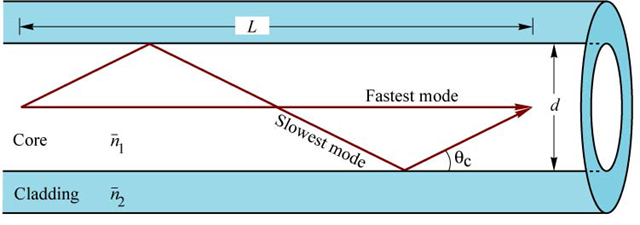
\includegraphics[scale=0.65]{img/modal_dispersion.png}
    \caption{Vidová disperze ve vícevidových optických
    vláknech}
    \label{fig:modal_dispersion}
\end{figure}

Jak je vidět, disperze má v~optice mnoho podob
a projevuje se různými způsoby, které nemusí
nutně souviset se separací složek světla
pomocí hranolu. Pro příklad, dříve zmíněná
vidová disperze nastavá i u~monochromatického
světla a nemá tedy nic společného s~chromatickou
disperzí, která nastává při lomu světla na optickém
hranolu.

\subsection{Disperzní médium a disperzní křivky}
Nejprve je nutné vysvětlit podstatu média bez
disperze a jak je možné na základě disperzní křivky
určit fázovou rychlost vlny, aby bylo později jasné,
jak, v~čem, a proč se disperzní médium liší.
Jako příklad média bez disperze lze uvést vakuum
pro elektromagnetické vlny~\cite{wiki_disp_rel}.
Typicky se také vzduch považuje za médium bez
disperze pro viditelné spektrum světla, což
však není tak úplně pravda. Ve skutečnosti i
vzduch způsobuje disperzi světla, která je ovšem
tak nepatrná, že dle~\cite{air_dispersive} není
za většiny běžných situací lidským okem viditelná.
Pro představu je na obrázku~\ref{fig:air_disp}
zobrazena křivka udávající index lomu vzduchu
podle konkrétní vlnové délky za určitých standardních
podmínek, viz~\cite{air_dispersive}.
\begin{figure}[htbp]
    \centering
    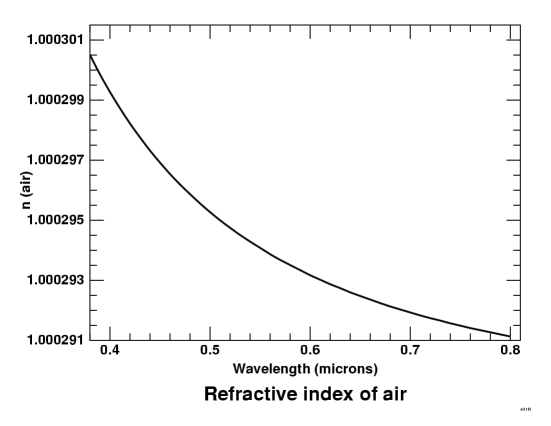
\includegraphics[scale=0.4]{img/disp_air.png}
    \caption{Disperzní křivka vzduchu}
    \label{fig:air_disp}
\end{figure}
Běžně se vzduch považuje za médium bez disperze
také pro zvukové vlny ve frekvenčním rozsahu,
který je slyšitelný lidským uchem. Nicméně vzduch
obsahuje molekuly $CO_2$ a je disperzní například
pro ultrazvuk~\cite{sound_dispersion}.

Obecně se disperzní závislost pro libovolný
fyzikální systém bez disperze získá vyřešením
následující vlnové rovnice, která ovšem popisuje
pouze situace, kdy máme jeden prostorový 
rozměr $x$:
$$
\frac{\partial^2 \psi}{\partial t^2}
   = c^2 \frac{\partial^2 \psi}{\partial x^2}.
$$
Člen $c \in \mathbb{R}$ je zde kladná konstanta,
která závisí na různých parametrech konkrétního
systému~\cite{wiki_wave_eq}. Řešením této rovnice
je libovolná funkce ve tvaru $f(x - ct)$, často
se ovšem řešení sestavují z~exponenciálních funkcí
následujícího tvaru:
$\psi(x,t) = Ae^{i(kx - \omega t)}$. Dosazením
exponenciální funkce tohoto tvaru do vlnové
rovnice získáme po úpravě následující triviální
disperzní závislost~\cite{harvard_disp}, která
odpovídá např. elektromagnetickým vlnám ve vakuu:
$$
\omega^2 = c^2k^2 \longrightarrow
\omega(k) = ck,
$$
kde $c$ je konstanta (nezávislá na $\omega$
i $k$) odpovídající
\textit{fázové rychlosti} vlny.
Triviální z~toho důvodu, že se jedná o~lineární
závislost, která odpovídá systému bez disperze,
jak uvidíme dále a jak je možné již vytušit
z~faktu, že $c$ je konstantní. Rychlost se nazývá
\textit{fázová}, abychom ji byli schopni odlišit
od \textit{grupové} rychlosti, kterou představíme
později, a také proto, že ve skutečnosti popisuje
jak rychle se u~sinusoidy $sin(kx - \omega t)$
pohybuje bod s~konstantní fází $kx - \omega t$.
Vztah pro fázovou rychlost je možné odvodit
následujícím způsobem:
$$
kx - \omega t = C \;\Longrightarrow\;
\frac{d(kx - \omega t)}{dt} = 0 \;\Longrightarrow\;
k\frac{dx}{dt} - \omega = 0 \;\Longrightarrow\;
\frac{dx}{dt} = \frac{\omega}{k} = v_f.
$$

Obrázek~\ref{fig:lin_disp_rel} obsahuje křivku
předchozí disperzní závislosti, která je lineární
a jedná se tedy o~přímku. Dále obrázek demonstruje,
že \textit{fázová} rychlost vlny graficky odpovídá
sklonu přímky procházející počátkem a konkrétním bodem
na přímce. Sklon přímky je dán její směrnicí, což
je v~tomto případě $c = \frac{\omega(k)}{k}$.
\begin{figure}[htbp]
\centering
\begin{tikzpicture}
\begin{axis}[xmax=5,ymax=5,samples=500,grid=major,
xlabel={k},ylabel={$\omega(k)$}, width=10cm, height=6.5cm,
minor tick num=1,
grid=major,
axis lines=middle,
enlargelimits={abs=0.5},
ytick={0,1,...,5},
ticklabel style={font=\tiny,fill=white},
legend style={at={(1.5,1)}},
]

\addplot[red, ultra thick, 
domain=0:5,
mark=none,
samples=200,
unbounded coords=jump] {x};

\addplot[blue, thick, mark=none, dashed]
coordinates {(4, 0) (4, 4)};

\addplot[blue, thick, mark=none, dashed]
coordinates {(0, 4) (4, 4)};

\addplot[blue, thick, mark=none, dashed]
coordinates {(2, 0) (2, 2)};

\addplot[blue, thick, mark=none, dashed]
coordinates {(0, 2) (2, 2)};

\addplot[blue, ultra thick, mark=none]
coordinates {(0, 0) (2, 2)};

\node[
    label={[shift={(-0.8, -0.1)}]$v_f = c = 1$},
    circle,
    fill,
    inner sep=2pt,
    blue] at (axis cs:4,4) {};
    
\node[
    label={[shift={(0.9,-0.8)}]$v_f = c = 1$},
    circle,
    fill,
    inner sep=2pt,
    blue] at (axis cs:2,2) {};

%\addlegendentry{Ne-disperzní médium}
\end{axis}
\end{tikzpicture}
\caption{Lineární disperzní závislost $\omega(k) = ck$}
\label{fig:lin_disp_rel}
\end{figure}
Jak můžeme dále vidět, pro libovolný bod na této
křivce získáváme stejný poměr $\frac{\omega(k)}{k}$
a tedy i stejnou fázovou rychlost $v_f$, která je
konstantní a nezávislá na úhlové frekvenci či
vlnovém číslu. Zobrazená křivka tedy opravdu odpovídá
médiu bez disperze. Z~toho dále vyplývá, že ať
už máme jakkoliv složitý pulz (nebo vlnu), tak
\textit{fázová} rychlost libovolné
složky z~mnoha harmonických složek nám popisuje i
společnou rychlost celého pulzu a není tedy potřeba
zavádět nový druh rychlosti.

Problém ovšem nastává, pokud pracujeme se systémem,
který zahrnuje disperzi. Příkladem mohou být vlny
na tuhé struně, které popisuje následující vlnová
rovnice~\cite{yt_dispersion}:
$$
\frac{\partial^2 \psi}{\partial t^2}
   = \frac{T}{\mu} \cdot 
   \bigg(\frac{\partial^2 \psi}{\partial x^2} -
   \alpha \frac{\partial^4 \psi}{\partial x^4}
   \bigg),
$$
kde $T$ je síla napětí ve struně, $\mu$ je
hmotnost struny na jednotku délky a 
$\alpha \in \mathbb{R}$
je kladná konstanta odvíjející se od typu struny.
Řešením této vlnové rovnice je poté následující
vlnová funkce $\psi(x,t) = A\cos(kx - \omega t)$.
Po jejím dosazení do vlnové rovnice a dodatečných
úpravách získáváme tuto disperzní závislost:
$$
\omega^2 = \frac{T}{\mu}(k^2 + \alpha k^4)
\quad\longrightarrow\quad
\omega(k) = \sqrt{\frac{T}{\mu}} k 
\sqrt{1 + \alpha k^2}.
$$
Tato disperzní závislost je na první pohled
nelineární a její křivka pro konkrétní hodnoty
parametrů struny je zobrazena na
obrázku~\ref{fig:non_lin_disp_rel}.
\begin{figure}[htbp]
\centering
\begin{tikzpicture}
\begin{axis}[xmax=4,ymax=6,samples=500,grid=major,
xlabel={k},ylabel={$\omega(k)$}, width=8.5cm, height=8cm,
minor tick num=1,
grid=major,
axis lines=middle,
enlargelimits={abs=0.5},
ytick={0,1,...,6},
ticklabel style={font=\tiny,fill=white},
legend style={at={(1.5,1)}},
]

\addplot[red, ultra thick, 
domain=0:3.5,
mark=none,
samples=200,
unbounded coords=jump] {x * sqrt(1 + 0.2 * x^2)};

\addplot[blue, thick, mark=none, dashed]
coordinates {(3, 0) (3, {3 * sqrt(1 + 0.2 * 3^2)})};

\addplot[blue, thick, mark=none, dashed]
coordinates {(0, {3 * sqrt(1 + 0.2 * 3^2)}) 
(3, {3 * sqrt(1 + 0.2 * 3^2)})};

\addplot[blue, thick, mark=none, dashed]
coordinates {(2, 0) (2, {2 * sqrt(1 + 0.2 * 2^2)})};

\addplot[blue, thick, mark=none, dashed]
coordinates {(0, {2 * sqrt(1 + 0.2 * 2^2)}) 
(2, {2 * sqrt(1 + 0.2 * 2^2)})};

\addplot[blue, ultra thick, mark=none]
coordinates {(0, 0) (2, {2 * sqrt(1 + 0.2 * 2^2)})};

\addplot[blue, ultra thick, mark=none]
coordinates {(0, 0) (3, {3 * sqrt(1 + 0.2 * 3^2)})};

% \addplot[violet, ultra thick, mark=none]
% coordinates {(2, 0) (3, 0)};

% \addplot[violet, ultra thick, mark=none]
% coordinates {(0, {2 * sqrt(1 + 0.2 * 2^2)}) 
% (0, {3 * sqrt(1 + 0.2 * 3^2)})};

\node[
    circle,
    fill,
    inner sep=2pt,
    blue] at (axis cs:3,{3 * sqrt(1 + 0.2 * 3^2)}) {};
    
\node[
    circle,
    fill,
    inner sep=2pt,
    blue] at (axis cs:2,{2 * sqrt(1 + 0.2 * 2^2)}) {};

%\addlegendentry{Ne-disperzní médium}
\end{axis}
\end{tikzpicture}
\caption{Nelineární disperzní závislost $\omega(k) = 
\sqrt{\frac{T}{\mu}} k \sqrt{1 + \alpha k^2}$}
\label{fig:non_lin_disp_rel}
\end{figure}
Jak je vidět, pro různé body na křivce (různé
hodnoty úhlové frekvence) získáváme přímky
s~různými směrnicemi, což se graficky projeví
na sklonu přímky, který se pro každý bod na křivce
liší. Zároveň zde platí dříve odvozený vztah pro
lineární disperzní závislost a sklon přímky je
tedy opět roven \textit{fázové} rychlosti sinusoidy
s~danou frekvencí.

Otázkou ovšem je, zda je nyní možné nalézt nějakou
\uv{společnou} rychlost, která charakterizuje
vlnu s~dvěma a více harmonickými složkami, jestliže
se každá z~nich pohybuje vlastní rychlostí.
Odpověď je ano, přičemž tuto společnou rychlost
nazýváme \textit{grupovou}. Nyní si demonstrujeme,
jak je možné jednoduše odvodit vztah pro
grupovou rychlost složením pouhých dvou
sinusoid a jak je možné ji určit graficky
z~disperzní křivky. Uvažujme tedy, že máme
následující dvě vlny:
\begin{alignat*}{1}
\psi_1(x, t) &= A\cos(k_1x - \omega_1t)\\
\psi_2(x, t) &= A\cos(k_2x - \omega_2t)
\end{alignat*}
Jestliže tyto vlny složíme dohromady
s~využitím trigonometrického vzorečku:
$$
\cos \theta +\cos \varphi =2\cos \left({\frac {\theta +\varphi }{2}}\right)\cos \left({\frac {\theta -\varphi }{2}}\right),
$$
získáme následující složenou vlnu:
$$
\psi_1(x, t) + \psi_2(x, t) =
2A\cos\Big(\overline{k}x - \overline{\omega}t\Big)
\cos\Big(\frac{\Delta k}{2}x - 
\frac{\Delta\omega}{2}t\Big),
$$
kde $\overline{k} = \frac{k_1 + k_2}{2}$,
$\overline{\omega} = \frac{\omega_1 + \omega_2}{2}$,
$\Delta k = k_1 - k_2$ a 
$\Delta\omega = \omega_1 - \omega_2$.
Obrázek~\ref{fig:wave_sum} ukazuje prostorový
průběh této vlny s~parametry $k_1 = 10$ a
$k_2 = 8$ zachycený v~čase $t = 0$.
Z~obrázku je patrné, že výsledná vlna je
produktem dvou vln s~různými vlnovými
délkami, které jsou odlišné od původních
vlnových délek.
\begin{figure}[!ht]
\centering
\begin{minipage}{0.49\linewidth}
\centering
\begin{tikzpicture}
\begin{axis}[xmin=0, xmax=6, ymin=-2,
ymax=2,samples=500,grid=major,
xlabel={x},ylabel={y}, width=8.8cm, height=7cm,
minor tick num=1,
grid=major,
axis lines=middle,
enlargelimits={abs=0.5},
ytick={-2,-1,...,2},
ticklabel style={font=\tiny,fill=white},
legend style={at={(1,1)}},
]

\addplot[blue, ultra thick, 
domain=0:6,
mark=none,
samples=200,
unbounded coords=jump] {cos(deg(9*x)) *
cos(deg(-x))};

\addplot[red, ultra thick, dashed,
domain=0:6,
mark=none,
samples=200,
unbounded coords=jump] {cos(deg(x))};

\addlegendentry{$cos(9x)cos(x)$}
\addlegendentry{$cos(x)$}

\end{axis}
\end{tikzpicture}
\end{minipage}
\hfill
\begin{minipage}{0.49\linewidth}
\centering
\begin{tikzpicture}
\begin{axis}[xmin=0, xmax=6, ymin=-2,
ymax=2,samples=500,grid=major,
xlabel={x},ylabel={y}, width=8.8cm, height=7cm,
minor tick num=1,
grid=major,
axis lines=middle,
enlargelimits={abs=0.5},
ytick={-2,-1,...,2},
ticklabel style={font=\tiny,fill=white},
legend style={at={(1,1)}},
]

\addplot[blue, ultra thick, 
domain=0:6,
mark=none,
samples=200,
unbounded coords=jump] {cos(deg(9*x))};

\addlegendentry{$cos(9x)$}

\end{axis}
\end{tikzpicture}
\end{minipage}
\caption{Moment složené vlny pro časový
okamžik $t = 0$}
\label{fig:wave_sum}
\end{figure}

Složka
$\cos\Big(\frac{\Delta k}{2}x - 
\frac{\Delta\omega}{2}t\Big)$
odpovídá červené, pomalu se měnící vlně.
Její rychlost šíření v~čase lze odvodit
stejným způsobem jako dříve pomocí obecného
vzorce pro rychlost šíření sinusoidy:
$$
\frac{dx}{dt} = \frac{\omega}{k} = v
\quad\longrightarrow\quad
v_1 = \frac{\frac{\Delta\omega}{2}}
{\frac{\Delta k}{2}} = 
\frac{\Delta\omega}{\Delta k}
$$
Pro tento konkrétní příklad lze rychlost $v_1$
označit za grupovou, přičemž k~obecnějšímu a
běžně používanému vztahu pro grupovou rychlost
se dopracujeme za chvíli. Červená vlna svým
způsobem provádí 
\uv{amplitudovou modulaci} a často se označuje
jako \textit{obálka} výsledné vlny. Naopak složka
$\cos\Big(\overline{k}x - \overline{\omega}t\Big)$
odpovídá modré, rychle se měnící vlně, kterou lze
pozorovat v~pravém grafu obrázku~\ref{fig:wave_sum}.
Její rychlost $v_2$ odvodíme stejným způsobem a
v~tomto konkrétním příkladu odpovídá fázové
rychlosti složené vlny:
$v_2 = \frac{\overline{\omega}}{\overline{k}}$.

Pokud bychom se na okamžik vrátili zpět
k~médiu bez disperze, tak můžeme na
obrázku~\ref{fig:wave_sum_non_dispersive}
pozorovat, že rychlost šíření obou složek
je konstantní a shodná s~původními fázovými
rychlostmi obou vln:
$$
v_{f1} = v_{f2} = \frac{\omega_1}{k_1} =
\frac{\omega_2}{k_2} = 
\frac{\overline{\omega}}{\overline{k}} = v_2 =
\frac{\Delta\omega}{\Delta k} = v_1.
$$
\begin{figure}[htbp]
\centering
\begin{tikzpicture}
\begin{axis}[xmax=5,ymax=5,samples=500,grid=major,
xlabel={k},ylabel={$\omega(k)$}, width=10cm, height=7cm,
minor tick num=1,
grid=major,
axis lines=middle,
enlargelimits={abs=0.5},
ytick={0,1,...,5},
ticklabel style={font=\tiny,fill=white},
legend style={at={(1.5,1)}},
]

\addplot[red, ultra thick, 
domain=0:5,
mark=none,
samples=200,
unbounded coords=jump] {x};

\addplot[blue, thick, mark=none, dashed]
coordinates {(4, 0) (4, 4)};

\addplot[blue, thick, mark=none, dashed]
coordinates {(0, 4) (4, 4)};

\addplot[blue, thick, mark=none, dashed]
coordinates {(2, 0) (2, 2)};

\addplot[blue, thick, mark=none, dashed]
coordinates {(0, 2) (2, 2)};

\addplot[violet, ultra thick, mark=none]
coordinates {(2, 0) (4, 0)};

\addplot[violet, ultra thick, mark=none]
coordinates {(0, 2) (0, 4)};

\addplot[blue, thick, mark=none, dashed]
coordinates {(3, 0) (3, 3)};

\addplot[blue, thick, mark=none, dashed]
coordinates {(0, 3) (3, 3)};

\addplot[violet, ultra thick, mark=none]
coordinates {(2, 2) (4, 4)};
    
\node[
    label={
    [right,yshift=2.1ex,xshift=0.3em]180:
    {$\overline{k}$}},
    inner sep=2pt] at (axis cs:3,0) {};
    
\node[
    label={
    [right,yshift=2.1ex,xshift=0.3em]180:
    {$k_1$}},
    inner sep=2pt] at (axis cs:2,0) {};
    
\node[
    label={
    [right,yshift=2.1ex,xshift=0.3em]180:
    {$k_2$}},
    inner sep=2pt] at (axis cs:4,0) {};
    
\node[
    label={
    [right,yshift=0.5em,xshift=2.1ex]180:
    {$\overline{\omega}$}},
    inner sep=2pt] at (axis cs:0,3) {};
    
\node[
    label={
    [right,yshift=0.5em,xshift=2.1ex]180:
    {$\omega_1$}},
    inner sep=2pt] at (axis cs:0,2) {};
    
\node[
    label={
    [right,yshift=0.5em,xshift=2.1ex]180:
    {$\omega_2$}},
    inner sep=2pt] at (axis cs:0,4) {};
    
\node[
    label={
    [right, shift={(0,0.5em)}]180:
    {$\color{violet}\Delta\omega$}},
    inner sep=2pt] at (axis cs:2,3) {};
    
\node[
    label={
    [right, shift={(0,0.5em)}]180:
    {$\color{violet}\Delta k$}},
    inner sep=2pt] at (axis cs:3,2) {};

\end{axis}
\end{tikzpicture}
\caption{Fázová a grupová rychlost složené vlny
v~médiu bez disperze}
\label{fig:wave_sum_non_dispersive}
\end{figure}
To je opět dáno tím, že závislost je lineární
a poměr mezi průměrnými hodnotami pro rychlost
$v_2$ i mezi rozdíly pro rychlost $v_1$ je
totožný s~poměry mezi parametry původních vln
$\psi_1$ a $\psi_2$ což demonstruje
obrázek~\ref{fig:wave_sum_non_dispersive}.
Nyní uvažujme, že $k_1$ vlny $\psi_1$ je téměř
shodné s~$k_2$ vlny $\psi_2$, neboli 
$k_1 \approx k_2$, což znamená, že i
kruhové frekvence obou vln jsou téměř totožné
$\omega_1 \approx \omega_2$. Pak platí následující:
$$
\frac{k_1 + k_2}{2} \approx k_1 \approx k_2
\quad\land\quad
\frac{\omega_1 + \omega_2}{2}
\approx \omega_1 \approx \omega_2
\quad\longrightarrow\quad
v_2 =\frac{\overline{\omega}}{\overline{k}}
= \frac{\omega}{k} = v_{f1} = v_{f2}
$$
Tím jsme se dopracovali k~tomu, že
\textit{fázová} rychlost složené vlny
$v_2$ je v~podstatě shodná s~původními
fázovými rychlostmi vln $\psi_1$ a $\psi_2$.
Zajímavější je ovšem vztah pro rychlost
$v_1$. Pokud se $k_1$ limitně blíží ke
$k_2$, pak se $\Delta k$ limitně blíží
k~nule (to stejné platí i pro $\Delta\omega$)
a vzorec pro rychlost $v_2$ pak v~podstatě
odpovídá derivaci:
$$
\lim_{k_1\to k_2}\frac{\omega_1 - \omega_2}
{k_1 - k_2}
\quad\longrightarrow\quad
v_2 = \frac{\Delta\omega}{\Delta k} = 
\frac{d\omega}{dk} = v_g
$$
Derivace skutečně odpovídá obecnému vzorci
pro \textit{grupovou} rychlost a graficky
odpovídá sklonu (směrnici) tečny v~konkrétním
bodě disperzní křivky. Je tedy zřejmé, že pro
médium bez disperze je grupová rychlost sinusoidy
konstantní a shodná s~její fázovou rychlostí, což
ovšem neplatí pro disperzní médium viz
obrázek~\ref{fig:group_velocity}.
\begin{figure}[htbp]
\centering
\begin{tikzpicture}
\begin{axis}[xmax=3.5,ymax=6,samples=500,grid=major,
xlabel={k},ylabel={$\omega(k)$}, width=10cm, 
height=7cm,
minor tick num=1,
grid=major,
axis lines=middle,
enlargelimits={abs=0.5},
ytick={0,1,...,6},
ticklabel style={font=\tiny,fill=white},
legend style={at={(1.5,1)}},
]

\addplot[red, ultra thick, 
domain=0:3,
mark=none,
samples=200,
unbounded coords=jump] {x * sqrt(0.5 * x^2)};

\addplot[blue, ultra thick, mark=none]
coordinates {(0, 0) (2, {2 * sqrt(0.5 * 2^2)})};

\addplot[mygreen, ultra thick,
domain=1.3:2.7,
mark=none,
samples=200,
unbounded coords=jump] {2.82842*x
- (2 * sqrt(0.5 * 2^2))};
    
\node[
    circle,
    fill,
    inner sep=2pt,
    blue] at (axis cs:2,{2 * sqrt(0.5 * 2^2)}) {};

\end{axis}
\end{tikzpicture}
\caption{Vizuální reprezentace fázové a grupové
rychlosti vlny pro disperzní médium}
\label{fig:group_velocity}
\end{figure}

Mohou tedy nastat tři různé situace, které
se v~našem jednoduchém příkladu s~dvěma vlnami
projeví následovně:
\begin{itemize}
    \item $\bm{v_g > v_f}$:
    \textit{anomální disperze}, která
    vzniká pokud máme \textit{konvexní}
    disperzní křivku. Jednoduše řečeno
    odpovídá situaci, kdy se rychlost
    šíření vlny v~médiu zvyšuje se
    zvyšující se frekvencí. Červená
    vlna z~obrázku~\ref{fig:wave_sum}
    tvořící obálku se v~tomto případě
    šíří v~čase rychleji než modrá
    vlna. Modrá vlna ovšem stále
    respektuje tvar obálky.
    
    \item $\bm{v_g = v_f}$:
    médium bez disperze, neboli lineární
    disperzní závislost. Obě složky se
v~čase šíří stejnou rychlosti.
    
    \item $\bm{v_g < v_f}$:
    \textit{normální disperze}, která
    vzniká pokud máme \textit{konkávní}
    disperzní křivku. Tato varianta odpovídá
    situaci, kdy se rychlost šíření vlny
    v~médiu snižuje se zvyšující se frekvencí.
    Modrá vlna se v~tomto případě propaguje
    obálkou vyšší rychlostí a respektuje její
    tvar.
\end{itemize}

Jednotlivé varianty lze pozorovat na
obrázku~\ref{fig:dispersion_types}.
Zajímavá je například situace, kdy je křivka
klesající, což znamená, že \textit{grupová}
rychlost je záporná. To se projeví tak, že
obálka (červená vlna) se v~čase šíří ve
směru záporné osy $x$, přičemž modrá vlna
se stále pohybuje v~kladném směru osy $x$,
jelikož její rychlost je kladná.
\begin{figure}[htbp]
\centering
\begin{tikzpicture}
\begin{axis}[xmax=5,ymax=6,samples=500,grid=major,
xlabel={k},ylabel={$\omega(k)$}, width=12cm, 
height=8cm,
minor tick num=1,
grid=major,
axis lines=middle,
enlargelimits={abs=0.5},
ytick={0,1,...,6},
ticklabel style={font=\tiny,fill=white},
legend style={at={(1.20,1)},
nodes={scale=0.8, transform shape}}
]

\addplot[black, ultra thick,
domain=0:4,
mark=none,
samples=200,
unbounded coords=jump] {x};

\addplot[red, ultra thick, 
domain=0:4,
mark=none,
samples=200,
unbounded coords=jump] {x * sqrt(1 + 0.05 * x^2)};

\addplot[blue, ultra thick, 
domain=0:6,
mark=none,
samples=200,
unbounded coords=jump] {x * sqrt(1 - 0.05 * x^2)};

\addlegendentry{bez disperze}
\addlegendentry{anomální disperze}
\addlegendentry{normální disperze}

\end{axis}
\end{tikzpicture}
\caption{Typy disperze a jejich křivky}
\label{fig:dispersion_types}
\end{figure}
Tuto situaci
lze připodobnit ke známému tanečnímu pohybu
\textit{Moonwalk}, který proslavil Michael
Jackson, kdy je vytvořena iluze pohybu vpřed,
ovšem samotné tělo se stále pohybuje vzad.
Toto přirovnání je poměrně trefné, jelikož
v~praxi je právě \textit{grupová} rychlost to,
co nás zajímá, protože odpovídá rychlosti,
kterou se přenáší energie
vlněním~\cite{wiki_group_velocity} a tedy i
informace, pokud se bavíme například o~optických
kabelech. Grupová rychlost tedy nemůže být
větší než rychlost světla ve vakuu, na rozdíl
od fázové rychlosti, viz dále.

V~našem triviálním příkladu s~dvěma vlnami
bylo jednoznačné, pomocí které složky se
určí grupová rychlost. V~praxi se ovšem často
pracuje se složitějšími pulzy, které jsou tvořeny
složením mnoha harmonických složek a vyvstává
tak otázka, pro kterou frekvenci (vlnové číslo)
bychom měli vyhodnotit $v_g = \frac{d\omega}{k}$,
jelikož nejsme schopni nalézt jednu společnou
grupovou rychlost, jako tomu bylo možné v~našem
triviálním případě s~dvěma složkami.
Dle~\cite{harvard_disp} se často pro vyhodnocení
volí dominantní frekvence, kterou jsme schopni
nalézt pomocí Fourierovy transformace nad
daným pulzem.

Poslední zajímavostí je fakt, že při vhodné
disperzní závislosti je možné docílit toho,
že fázová rychlost vlny překročí rychlost
světla $c$. To nám ovšem nevadí, protože
ve skutečnosti nedochází k~přenosu energie
a není tak porušena teorie relativity. Aby
došlo k~přenosu energie, musíme způsobit změnu
ve vlně a každý takový signál se může šířit
pouze tak rychle jako čelní hrana této změny,
která již je limitována rychlostí světla.
Ve skutečnosti i grupová rychlost může ve
speciálních případech, jako je například
anomální disperze, překročit rychlost světla,
což nám ovšem opět nevadí, protože samotný
přenos energie tuto hranici nepřekročí.
Dokument~\cite{harvard_disp} poskytuje
detailnější popis této problematiky.


\subsection{Chromatická disperze}
Jedním z~nejznámějších projevů disperze je
separace jednotlivých složek polychromatického
světla pomocí hranolu z~vhodného disperzního
materiálu. Přesněji se jedná o~takzvanou
\textit{chromatickou} disperzi a separace světla
je pouze jejím důsledkem. Jak bylo ukázáno
v~předchozí kapitole, \textit{fázová} i
\textit{grupová} rychlost šíření vlny v~disperzním
prostředí je závislá na vlnové délce, případně
frekvenci vlny a můžeme tedy říci, že se ve
skutečnosti jedná o~funkce:
$v_p(\lambda)$, $v_g(\lambda)$. 
Tento fakt úzce souvisí s~vzorcem pro tzv.
\textit{absolutní} index lomu $n$, který udává poměr
mezi rychlostí šíření elektromagnetického vlnění ve
vakuu $c$ a rychlostí šíření v~libovolném jiném médiu $v$:
$n = \frac{c}{v}$.

Často se ovšem nespecifikuje,
že pro určení indexu lomu se využívá \textit{fázová}
rychlost vlny. Z~toho logicky vyplývá, že i
index lomu je pro disperzní média ve skutečnosti
funkcí vlnové délky a přesnější vzorec by tedy
mohl vypadat například následovně: 
$n(\lambda) = \frac{c}{v_p(\lambda)}$.
Pro lepší představu se často index lomu popisuje
jako koeficient udávající zpomalení oproti rychlosti
světla ve vakuu, pokud vyjádříme ze vzorce rychlost:
$v_p(\lambda) = \frac{c}{n(\lambda)}$. Index lomu
lze vyjádřit také pomocí poměru vlnových délek:
$n = \frac{\lambda_0}{\lambda}$, kde $\lambda_0$
je vlnová délka vlny ve vakuu a $\lambda$ je vlnová
délka v~daném médiu. Důležité je poznamenat, že při
přechodu z~jednoho média do druhého dochází ke změně
vlnové délky i rychlosti šíření tak, aby platil
vztah $v = \lambda f$, ale ke změně frekvence
vlnění \textit{nikdy} nedochází. To jsme schopni
pozorovat i prakticky, jelikož při lomu
monochromatického světla na hranolu nedochází ke
změně okem vnímané barvy, která je závislá právě
na frekvenci vlnění. Pro úplnost, vakuum má index
lomu roven $1$. Kromě klasického indexu lomu,
který je definován pro \textit{fázovou} rychlost
vlny, existuje i \textit{grupový index lomu}. Ten
je definován stejným způsobem jako klasický index
lomu, akorát pro \textit{grupovou} rychlost vlnění:
$n_g(\lambda) = \frac{c}{v_g(\lambda)}$.

V~minulé kapitole bylo zmíněno, že při vhodné
disperzní závislosti může fázová rychlost vlny
překonat rychlost světla, aniž by došlo k~porušení
teorie relativity, jelikož nedochází k~přenosu
informace. To ovšem znamená, že index lomu ve
skutečnosti může být nižší než $1$. Zajímavým
příkladem média s~takovým indexem lomu může být
ionosféra země, která je tvořena plazmatem.
Při vstupu vlny do takového média a refrakci
dochází k~odklonu vlnění od normály. 
Toho se využívá
například při rádiové komunikaci na velké
vzdálenosti~\cite{wiki_refractive_idx}.
Dokonce existují i materiály, jejichž index
lomu je záporný~\cite{wiki_negative_index}
a dochází tak k~negativní refrakci, se kterou
se běžně nesetkáváme.

Klíčové pro separaci barev ovšem je, že
index lomu ovlivňuje úhel lomu při přechodu
vlnění z~jednoho prostředí do druhého. Jelikož
index lomu závisí na vlnové délce, pak i samotný
uhel lomu je závislý na vlnové délce, což ve
výsledku způsobuje dříve zmíněnou a dobře známou
separaci bílého světla na jednotlivé složky při
průchodu hranolem pod vhodným úhlem. Opět je vhodné
zdůraznit, že \textit{disperzí} nazýváme konkrétně
závislost indexu lomu na vlnové délce a separace
složek světla je pouze jedním z~\textit{důsledků}
disperze. Dalším a tentokrát nepříjemným příkladem
důsledků disperze je závislost ohniskové vzdálenosti
čočky na vlnové délce. Tento jev je jedním z~typů
tzv. \textit{chromatické aberace}~\cite{wiki_aberration},
což je ve většině případů nežádoucí efekt, 
který se často musí různými způsoby (například i
pomocí software) alespoň částečně eliminovat.
Na obrázku~\ref{fig:aberration} můžeme pozorovat
praktický projev aberace, kdy jednotlivé barevné
složky měly při pořízení fotky posunuté ohniska, což
způsobilo rozostření a separaci barev na výsledné fotce.
\begin{figure}[htbp]
    \centering
    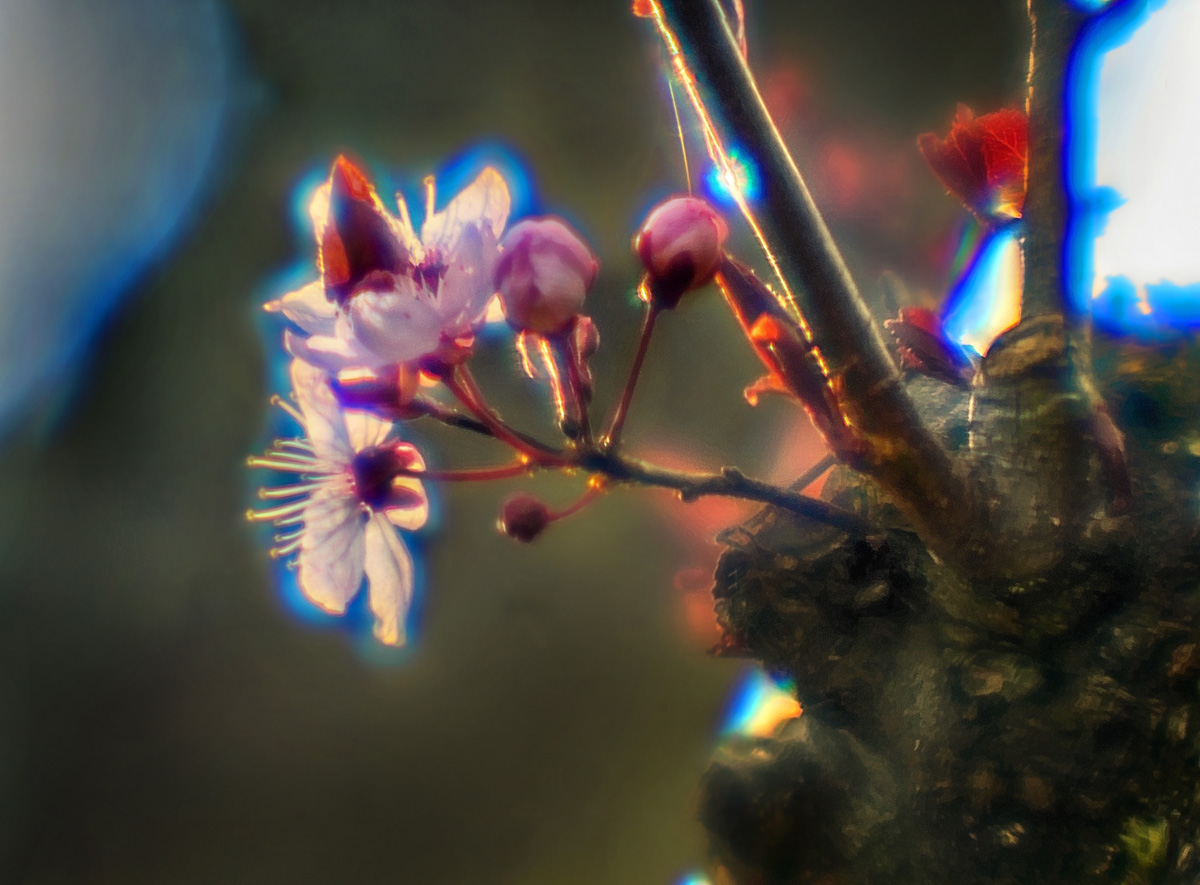
\includegraphics[scale=0.20]{img/aberration.jpeg}
    \caption{Chromatická aberace v~praxi. Při
    pořízení fotky byly použity čočky zvýrazňující
    efekt aberace.}
    \label{fig:aberration}
\end{figure}

Jak konkrétně se světlo na rozhraní mezi prostředími
láme lze poté určit pomocí tzv. 
\textit{Snellova zákona}~\cite{wiki_snells_law}, 
který popisuje vztah mezi
úhlem dopadu a lomu při přechodu vlnění z~jednoho
prostředí s~indexem lomu $n_1$ do druhého prostředí
s~indexem lomu $n_2$. Konkrétně, pokud paprsek při
dopadu na rozhraní svírá s~normálou povrchu úhel
$\theta_1$, pak úhel $\theta_2$, který bude svírat
lomený paprsek lze vypočítat pomocí následujícího
Snellova zákona:
$$
\frac{\sin\theta_2}{\sin\theta_1} = \frac{v_2}{v_1}
= \frac{n_1}{n_2}
\quad\longrightarrow\quad
\theta_2 = \arcsin\Big(\frac{n_1}{n_2}\sin\theta_1\Big)
$$
Na obrázku~\ref{fig:snell_law} lze pozorovat situaci,
která nastane, pokud světlo přechází z~tzv. opticky
řidšího prostředí do opticky hustšího, což znamená,
že $n_2 > n_1$.
\begin{figure}[htbp]
    \centering
    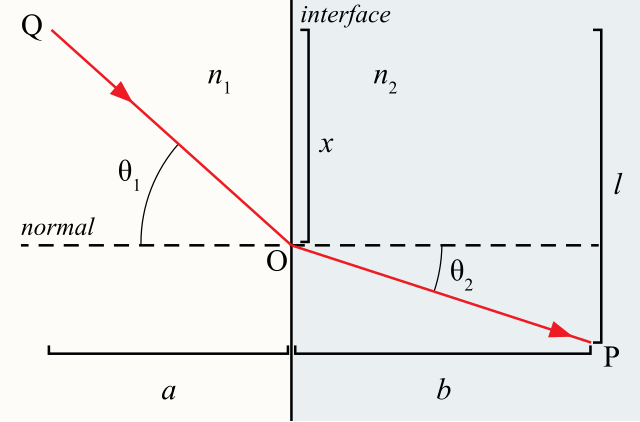
\includegraphics[scale=0.37]{img/snells_law.png}
    \caption{Přechod paprsku z~opticky řidšího
    prostředí do opticky hustšího. Úhel lomu
    $\theta_2$ lze vypočítat pomocí Snellova zákona.}
    \label{fig:snell_law}
\end{figure}
V~tomto případě se světlo láme směrem k~normále,
ale pokud bychom měli opačný případ, kdy $n_1 > n_2$,
pak by se světlo lámalo naopak směrem od normály.
Kromě toho nám Snellův zákon slouží také k~určení
tzv. úhlu totálního odrazu. Totální odraz je jev,
při kterém dochází k~odrazu veškerého dopadajícího
světla, pokud jsou splněny dvě podmínky:
\begin{enumerate}
    \item Vlnění přechází z~prostředí opticky
    hustšího do prostředí opticky řidšího,
    $n_1 > n_2$.
    
    \item Úhel, který dopadající paprsek svírá
    s~normálou je větší než tzv. \textit{kritický
    úhel} $\theta_c$
\end{enumerate}
Úplného odrazu se v~optice hojně využívá, zejména
v~optických kabelech, které by bez úplného odrazu
nemohly fungovat. Výpočet kritického úhlu $\theta_c$
je založen na principu, že Snellův zákon by v~některých
případech vyžadoval, aby sinus úhlu lomu byl 
větší než $1$, což samozřejmě není možné. V~takových
případech k~lomu nedochází a místo toho dochází
k~úplnému odrazu na rozhraní. Pro výpočet kritického
úhlu stačí spočítat hodnotu úhlu $\theta_1$,
pro kterou je úhel $\theta_2$ roven $90^\circ$:
$$
\theta_c = \arcsin\Big(\frac{n_2}{n_1}
\sin\theta_2\Big) = \arcsin\frac{n_2}{n_1},
$$
kde $\sin\theta_2 = \sin(90^\circ) = 1$.
Kritický úhel vlastně odpovídá největšímu možnému
úhlu dopadu, kdy ještě dojde k~lomu světla, přičemž
v~tomto případě se lomený paprsek šíří na rozhraní
obou prostředí. Obrázek~\ref{fig:critical_angle}
demonstruje tři možné situace, které mohou nastat.
\begin{figure}[htbp]
    \centering
    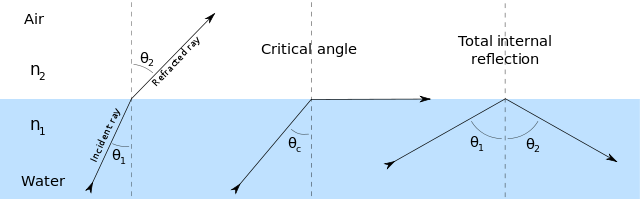
\includegraphics[scale=0.58]{img/critical_angle.png}
    \caption{Tři možné situace při přechodu světla
    z~opticky hustšího do opticky řidšího prostředí.}
    \label{fig:critical_angle}
\end{figure}

S~těmito znalostmi by již mělo být jasné, proč
dochází k~separaci barev bílého světla na hranolu
a jak můžeme jednoduše určit úhel lomu jednotlivých
barev.
\begin{figure}[htbp]
    \centering
    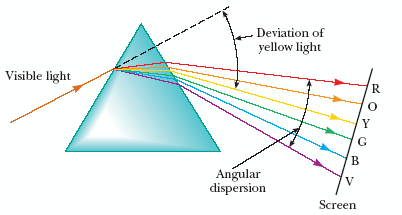
\includegraphics[scale=0.2]{img/prism.png}
    \caption{Separace bílého světla pomocí hranolu;
    znázornění \textit{úhlu deviace} a
    \textit{disperzního úhlu}, který svírá
    paprsek červeného světla s~paprskem
    fialového světla.}
    \label{fig:prism}
\end{figure}
Obrázek~\ref{fig:prism} ilustruje tuto situaci
a je vidět, že červené světlo s~největší vlnovou
délkou má nejvyšší úhel lomu (nejmenší úhel
deviace). Naopak fialové světlo s~nejmenší
vlnovou délkou má nejmenší úhel lomu (největší
úhel deviace). Jakým způsobem a jak moc se
světlo bude lámat opět záleží na konkrétním
materiálu a zda $n_1 > n_2$ nebo naopak.
U~běžných materiálů s~\textit{normální disperzí}
jako je sklo, se index lomu snižuje se zvyšující
se vlnovou délkou a úhel lomu se tím pádem
zvyšuje. Pokud bychom měli hranol z~materiálu
s~\textit{anomální disperzí}, pak by bylo pořadí
barev otočené.

Často potřebujeme znát \textit{úhel deviace}
paprsku,
případně \textit{disperzní úhel}, což je úhel,
který svírají paprsky s~extrémními úhly deviace
(minimální / maximální pro všechny obsažené
vlnové délky v~bílém světle),
v~našem případě červený a fialový paprsek na
obrázku~\ref{fig:prism}.
Vzorec pro úhel deviace lze odvodit na
základě geometrických vlastností hranolu,
trojúhelníku a čtyřúhelníku,
viz~\cite{ray_optics}[str. 331], kde je vzorec detailně
odvozen. Výsledný vzorec pro úhel deviace
$\delta$ vypadá následovně:
$\delta = i + e - \alpha$, kde $i$ je úhel
dopadu paprsku vstupujícího do hranolu,
$e$ je úhel lomu paprsku opouštějícího hranol
a $\alpha$ je vrcholový úhel hranolu.

Vrcholový úhel $\alpha$ i úhel dopadu $i$
známe, ale neznáme úhel lomu $e$, který je
potřeba vypočíst. Výpočet tohoto úhlu je
založený na jednoduchém trasování paprsku a využití
Snellova zákona. Obrázek~\ref{fig:prism_deviation}
demonstruje průchod červeného paprsku hranolem a
popisuje veškeré úhly, které jsou při výpočtu
potřeba. V~tomto případě platí $i = \theta_0$
a $e = \theta'_1$.
\begin{figure}[htbp]
    \centering
    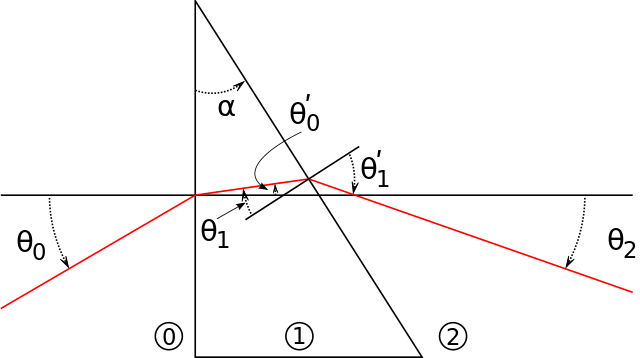
\includegraphics[scale=0.4]{img/prism_deviation.png}
    \caption{Refrakce paprsku při průchodu hranolem}
    \label{fig:prism_deviation}
\end{figure}
Paprsek nejprve dopadá na první rozhraní pod
úhlem $\theta_0$ a dochází k~refrakci. Úhel
$\theta'_0$ lomeného paprsku proto spočteme
následovně:
$$
\theta'_0 = \arcsin\Big(\frac{n_0}{n_1}
\sin\theta_0\Big),
$$
kde $n_0$ je index lomu média nalevo od hranolu
a $n_1$ je index lomu hranolu. Pomocí geometrie
se dále můžeme dopracovat k~následujícímu vzorci pro
druhý úhel dopadu $\theta_1 = \alpha - \theta'_0$.
Jakmile známe druhý úhel dopadu, můžeme opětovně
aplikovat Snellův zákon a získat druhý úhel lomu:
$$
\theta'_1 = \arcsin\Big(\frac{n_1}{n_2}
\sin\theta_1\Big).
$$
Výsledný úhel deviace $\delta$ je roven
součtu úhlů $\theta_0$ a $\theta_2$, kde
$\theta_2 = \theta'_1 - \alpha$, což odpovídá
obecnému vzorci $\delta = i + e - \alpha$.
Pro získání finálního vzorce tedy stačí
složit dohromady odvozené rovnice, přičemž pro
zjednodušení uvažujeme, že $n_0 = n_2$:
$$
\delta = \theta_0 + \theta_2 =
\theta_0 + \arcsin\Big(
\frac{n_1}{n_0}\sin\Big[
\alpha - \arcsin\Big(
\frac{n_0}{n_1}\sin\theta_0
\Big)\Big]\Big) - \alpha
$$

Důležité je uvědomit si, že indexy lomu použité
v~rovnicích jsou ve skutečnosti opět funkcemi
vlnové délky a zde byly pouze pro lepší čitelnost
zvoleny indexy lomu $n_0$, $n_1$ a $n_2$ pro
konkrétní vlnové délky. Konečně, pro určení
\textit{disperzního úhlu} pak stačí pouze odečíst
od největšího dosaženého úhlu deviace nejmenší
dosažený úhel deviace jak bylo zmíněno dříve,
tedy $\Phi = \delta_{max} - \delta_{max}$.
Na obrázku~\ref{fig:prism} se jedná o~úhly
deviace fialového a červeného paprsku, ale
v~obecném případě se jedná o~maximální a minimální
úhly, jelikož opět záleží na zvoleném materiálu,
který může způsobovat anomální disperzi.


\subsection{Využití disperze}
Přestože jsou projevy disperze v~mnoha
situacích, jako například u~optických vláken,
nežádoucí a je nutné je různými způsoby
zmírňovat či dokonce eliminovat, existuje
mnoho aplikací, pro které jsou projevy
disperze naopak klíčové.

Obecně se disperze využívá ve spektroskopii,
což je studium interakce mezi hmotou a
elektromagnetickým zářením~\cite{wiki_spectroscopy}.
Existují různé
druhy spektroskopie, které se odvíjí například
od toho, jaké části elektromagnetického spektra
se při experimentech využívají. Velmi důležitá
je potom tzv. infračervená (IR) spektroskopie,
která je klíčová zejména pro studium látek
v~organické chemii. Velmi zjednodušeně se využívá
toho, že molekuly absorbují určité frekvence
v~závislosti na tom, jaká je jejich struktura.
Typický spektroskopický experiment poté spočívá
v~systematickém ozařování daného studovaného
vzorku (látky) pomocí elektromagnetických vln
s~rozdílnými frekvencemi (souvisí s~energií
záření). Různé frekvence záření jsou poté
hmotou různě ovlivněny a dochází k~emisi
světla. Toto světlo je poté zachycováno na
detektoru, který produkuje tzv. emisní spektrum
jež se dále studuje.

Součástí detektoru je poté buď spektrometr
a nebo spektrograf, což jsou nástroje, které
přímo využívají disperzního jevu pro separaci
světla na jednotlivé složky o~různých frekvencích,
čímž produkují požadované spektrum. Dříve se
pro tyto účely využívalo jednoduchých optických
hranolů, které byly později nahrazeny tzv.
difrakčními mřížkami.

Technika spektroskopie je velmi rozmanitá a
má využití v~mnoha dalších odvětvích jako
například v~biomedicíně,
či astronomii při studiu složení hvězd, přičemž
na pozadí vždy v~nějaké podobě figuruje disperzní
jev. Dalo by se tedy říci, že spektroskopie
obecně je jednou z~hlavních aplikací disperzního
jevu.


\section{Demonstrační program}
Součástí tohoto semestrálního projektu
byla implementace programu, který vhodným
způsobem interaktivně demonstruje disperzní
jev a umožňuje uživateli experimentovat
s~různými parametry daného optického systému.
Konkrétně byla implementována vizualizace
chromatické disperze z~pohledu paprskové
optiky, jelikož se pravděpodobně jedná
o~nejznámější a nejnázornější projev disperze
světla v~optice.

Jádrem projektu je implementace algoritmu
sledování paprsku, který může procházet
různými optickými hranoly s~různými disperzními
vlastnostmi. Uživatel může manipulovat
s~počátkem či orientací jednotlivých paprsků
a nastavovat jejich vlnové délky. Dále
je možné manipulovat s~velikostí, pozicí
a rotací optických hranolů a
měnit body disperzní křivky materiálů
hranolů i prostředí.
Díky tomu lze nasimulovat jak normální,
tak anomální disperzi, vnější i vnitřní
úplný odraz a obecně i chování, které
běžné existující materiály nevykazují.
Index lomu mezi jednotlivými body disperzní
křivky je lineárně interpolován, což sice
neodpovídá žádnému reálnému materiálu,
nicméně pro účely demonstrace disperzního
jevu je snad dostačující.

Program je z~důvodu jednoduché přenositelnosti
implementován jako webová aplikace v~jazyce
\textit{JavaScript} s~využitím knihovny
\textit{PixiJS}, která slouží pro efektivní
vykreslování na \textit{HTML5} plátno s~využitím \textit{WebGL} API a grafické karty na pozadí.

\section{Záver}
V~rámci této práce byl nejprve obecně
představen disperzní jev a jeho nejčastější
projevy v~optice. Dále se text poměrně
detailně zabývá problematikou disperzních
médií a křivek, fázovou a grupovou rychlosti
a jejich spojitostí s~disperzí. Dále se
text zabývá konkrétně chromatickou
disperzí, Snellovým zákonem lomu a separací
polychromatického světla na optickém hranolu.
Závěr práce je věnován krátkému přehledu
praktických aplikací disperze v~různých vědních
oborech.

  
  % Kompilace po částech (viz výše, nutno odkomentovat)
  % Compilation piecewise (see above, it is necessary to uncomment it)
  %\subfile{projekt-01-uvod-introduction}
  % ...
  %\subfile{chapters/projekt-05-conclusion}


  % Pouzita literatura / Bibliography
  % ----------------------------------------------
\ifslovak
  \makeatletter
  \def\@openbib@code{\addcontentsline{toc}{chapter}{Literatúra}}
  \makeatother
  \bibliographystyle{bib-styles/slovakiso}
\else
  \ifczech
    \makeatletter
    \def\@openbib@code{\addcontentsline{toc}{chapter}{Literatura}}
    \makeatother
    \bibliographystyle{bib-styles/czechiso}
  \else 
    \makeatletter
    \def\@openbib@code{\addcontentsline{toc}{chapter}{Bibliography}}
    \makeatother
    \bibliographystyle{bib-styles/englishiso}
  %  \bibliographystyle{alpha}
  \fi
\fi
  \begin{flushleft}
  \bibliography{projekt-20-literatura-bibliography}
  \end{flushleft}

  % vynechani stranky v oboustrannem rezimu
  % Skip the page in the two-sided mode
  \iftwoside
    \cleardoublepage
  \fi

  % Prilohy / Appendices
  % ---------------------------------------------
  \appendix
\ifczech
  \renewcommand{\appendixpagename}{Přílohy}
  \renewcommand{\appendixtocname}{Přílohy}
  \renewcommand{\appendixname}{Příloha}
\fi
\ifslovak
  \renewcommand{\appendixpagename}{Prílohy}
  \renewcommand{\appendixtocname}{Prílohy}
  \renewcommand{\appendixname}{Príloha}
\fi
%  \appendixpage

% vynechani stranky v oboustrannem rezimu
% Skip the page in the two-sided mode
%\iftwoside
%  \cleardoublepage
%\fi
  
\ifslovak
%  \section*{Zoznam príloh}
%  \addcontentsline{toc}{section}{Zoznam príloh}
\else
  \ifczech
%    \section*{Seznam příloh}
%    \addcontentsline{toc}{section}{Seznam příloh}
  \else
%    \section*{List of Appendices}
%    \addcontentsline{toc}{section}{List of Appendices}
  \fi
\fi
  \startcontents[chapters]
  \setlength{\parskip}{0pt}
  % seznam příloh / list of appendices
  % \printcontents[chapters]{l}{0}{\setcounter{tocdepth}{2}}
  
  \ifODSAZ
    \setlength{\parskip}{0.5\bigskipamount}
  \else
    \setlength{\parskip}{0pt}
  \fi
  
  % vynechani stranky v oboustrannem rezimu
  \iftwoside
    \cleardoublepage
  \fi
  
  % Přílohy / Appendices
  %% Tento soubor nahraďte vlastním souborem s přílohami (nadpisy níže jsou pouze pro příklad)
% This file should be replaced with your file with an appendices (headings below are examples only)

% Umístění obsahu paměťového média do příloh je vhodné konzultovat s vedoucím
% Placing of table of contents of the memory media here should be consulted with a supervisor
%\chapter{Obsah přiloženého paměťového média}

%\chapter{Manuál}

%\chapter{Konfigurační soubor} % Configuration file

%\chapter{RelaxNG Schéma konfiguračního souboru} % Scheme of RelaxNG configuration file

%\chapter{Plakát} % poster

\chapter{Jak pracovat s touto šablonou}
\label{jak}

V této příloze je uveden popis jednotlivých částí šablony, po kterém následuje stručný návod, jak s touto šablonou pracovat. Pokud po jejím přečtení k šabloně budete mít nějaké dotazy, připomínky apod., neváhejte a napište na e-mail sablona@fit.vutbr.cz.

\section*{Popis částí šablony}

Po rozbalení šablony naleznete následující soubory a adresáře:
\begin{DESCRIPTION}
  \item [bib-styles] Styly literatury (viz níže). 
  \item [obrazky-figures] Adresář pro Vaše obrázky. Nyní obsahuje placeholder.pdf (tzv. TODO obrázek, který lze použít jako pomůcku při tvorbě technické zprávy), který se s prací neodevzdává. Název adresáře je vhodné zkrátit, aby byl jen ve zvoleném jazyce.
  \item [template-fig] Obrázky šablony (znak VUT).
  \item [fitthesis.cls] Šablona (definice vzhledu).
  \item [Makefile] Makefile pro překlad, počítání normostran, sbalení apod. (viz níže).
  \item [projekt-01-kapitoly-chapters.tex] Soubor pro Váš text (obsah nahraďte).
  \item [projekt-20-literatura-bibliography.bib] Seznam literatury (viz níže).
  \item [projekt-30-prilohy-appendices.tex] Soubor pro přílohy (obsah nahraďte).
  \item [projekt.tex] Hlavní soubor práce -- definice formálních částí.
\end{DESCRIPTION}

Výchozí styl literatury (czechiso) je od Ing. Martínka, přičemž slovenská a anglická verze (slovakiso a englishiso) jsou jeho překlady s drobnými modifikacemi. Oproti normě jsou v~něm určité odlišnosti, ale na FIT je dlouhodobě akceptován. Alternativně můžete využít styl od Ing. Radima Loskota nebo od Ing. Radka Pyšného\footnote{BP Ing. Radka Pyšného \url{http://www.fit.vutbr.cz/study/DP/BP.php?id=7848}}. Alternativní styly obsahují určitá vylepšení, ale zatím nebyly řádně otestovány větším množstvím uživatelů. Lze je považovat za beta verze pro zájemce, kteří svoji práci chtějí mít dokonalou do detailů a neváhají si nastudovat detaily správného formátování citací, aby si mohli ověřit, že je vysázený výsledek v pořádku.

\begin{samepage}
Makefile kromě překladu do PDF nabízí i další funkce:
\begin{itemize}
  \item přejmenování souborů (viz níže),
  \item počítání normostran,
  \item spuštění vlny pro doplnění nezlomitelných mezer,
  \item sbalení výsledku pro odeslání vedoucímu ke kontrole (zkontrolujte, zda sbalí všechny Vámi přidané soubory, a případně doplňte).
\end{itemize}
\end{samepage}

Nezapomeňte, že vlna neřeší všechny nezlomitelné mezery. Vždy je třeba manuální kontrola, zda na konci řádku nezůstalo něco nevhodného -- viz Internetová jazyková příručka\footnote{Internetová jazyková příručka \url{http://prirucka.ujc.cas.cz/?id=880}}.

\paragraph {Pozor na číslování stránek!} Pokud má obsah 2 strany a na 2. jsou jen \uv{Přílohy} a~\uv{Seznam příloh} (ale žádná příloha tam není), z nějakého důvodu se posune číslování stránek o 1 (obsah \uv{nesedí}). Stejný efekt má, když je na 2. či 3. stránce obsahu jen \uv{Literatura} a~je možné, že tohoto problému lze dosáhnout i jinak. Řešení je několik (od~úpravy obsahu, přes nastavení počítadla až po sofistikovanější metody). \textbf{Před odevzdáním proto vždy překontrolujte číslování stran!}


\section*{Doporučený postup práce se šablonou}

\begin{enumerate}
  \item \textbf{Zkontrolujte, zda máte aktuální verzi šablony.} Máte-li šablonu z předchozího roku, na stránkách fakulty již může být novější verze šablony s~aktualizovanými informacemi, opravenými chybami apod.
  \item \textbf{Zvolte si jazyk}, ve kterém budete psát svoji technickou zprávu (česky, slovensky nebo anglicky) a svoji volbu konzultujte s vedoucím práce (nebyla-li dohodnuta předem). Pokud Vámi zvoleným jazykem technické zprávy není čeština, nastavte příslušný parametr šablony v souboru projekt.tex (např.: \verb|documentclass[english]{fitthesis}| a přeložte prohlášení a poděkování do~angličtiny či slovenštiny.
  \item \textbf{Přejmenujte soubory.} Po rozbalení je v šabloně soubor \texttt{projekt.tex}. Pokud jej přeložíte, vznikne PDF s technickou zprávou pojmenované \texttt{projekt.pdf}. Když vedoucímu více studentů pošle \texttt{projekt.pdf} ke kontrole, musí je pracně přejmenovávat. Proto je vždy vhodné tento soubor přejmenovat tak, aby obsahoval Váš login a (případně zkrácené) téma práce. Vyhněte se však použití mezer, diakritiky a speciálních znaků. Vhodný název může být např.: \uv{\texttt{xlogin00-Cisteni-a-extrakce-textu.tex}}. K přejmenování můžete využít i přiložený Makefile:
\begin{verbatim}
make rename NAME=xlogin00-Cisteni-a-extrakce-textu
\end{verbatim}
  \item Vyplňte požadované položky v souboru, který byl původně pojmenován \texttt{projekt.tex}, tedy typ, rok (odevzdání), název práce, svoje jméno, ústav (dle zadání), tituly a~jméno vedoucího, abstrakt, klíčová slova a další formální náležitosti.
  \item Nahraďte obsah souborů s kapitolami práce, literaturou a přílohami obsahem svojí technické zprávy. Jednotlivé přílohy či kapitoly práce může být výhodné uložit do~samostatných souborů -- rozhodnete-li se pro toto řešení, je doporučeno zachovat konvenci pro názvy souborů, přičemž za číslem bude následovat název kapitoly. 
  \item Nepotřebujete-li přílohy, zakomentujte příslušnou část v \texttt{projekt.tex} a příslušný soubor vyprázdněte či smažte. Nesnažte se prosím vymyslet nějakou neúčelnou přílohu jen proto, aby daný soubor bylo čím naplnit. Vhodnou přílohou může být obsah přiloženého paměťového média.
  \item Zadání, které si stáhnete v PDF z IS FIT (odkaz \uv{Zadání pro vložení do práce} či \uv{Thesis assignment}), uložte do souboru \texttt{zadani.pdf} a povolte jeho vložení do práce parametrem šablony v \texttt{projekt.tex} (\verb|documentclass[zadani]{fitthesis}|).
  \item Nechcete-li odkazy tisknout barevně (tedy červený obsah -- bez konzultace s vedoucím nedoporučuji), budete pro tisk vytvářet druhé PDF s tím, že nastavíte parametr šablony pro tisk: (\verb|documentclass[zadani,print]{fitthesis}|). Budete-li tisknout barevně, místo \texttt{print} použijte parametr \texttt{cprint}. Barevné logo se nesmí tisknout černobíle!
  \item Vzor desek, do kterých bude práce vyvázána, si vygenerujte v informačním systému fakulty u zadání. Pro disertační práci lze zapnout parametrem v šabloně \texttt{cover} (více naleznete v souboru \texttt{fitthesis.cls}).
  \item Nezapomeňte, že zdrojové soubory i (obě verze) PDF musíte odevzdat na CD či jiném médiu přiloženém k technické zprávě.
\end{enumerate}

Obsah práce se generuje standardním příkazem \tt \textbackslash tableofcontents \rm (zahrnut v šabloně). Přílohy jsou v něm uvedeny úmyslně.

\subsection*{Pokyny pro oboustranný tisk}
\begin{itemize}
\item \textbf{Oboustranný tisk je doporučeno konzultovat s vedoucím práce.}
\item Je-li práce tištěna oboustranně a její tloušťka je menší než tloušťka desek, nevypadá to dobře.
\item Zapíná se parametrem šablony: \verb|\documentclass[twoside]{fitthesis}|
\item Po vytištění oboustranného listu zkontrolujte, zda je při prosvícení sazební obrazec na obou stranách na stejné pozici. Méně kvalitní tiskárny s duplexní jednotkou mají často posun o 1--3 mm. Toto může být u některých tiskáren řešitelné tak, že vytisknete nejprve liché stránky, pak je dáte do stejného zásobníku a vytisknete sudé.
\item Za titulním listem, obsahem, literaturou, úvodním listem příloh, seznamem příloh a případnými dalšími seznamy je třeba nechat volnou stránku, aby následující část začínala na liché stránce (\textbackslash cleardoublepage).
\item  Konečný výsledek je nutné pečlivě překontrolovat.
\end{itemize}

\subsection*{Styl odstavců}

Odstavce se zarovnávají do bloku a pro jejich formátování existuje více metod. U papírové literatury je častá metoda s~použitím odstavcové zarážky, kdy se u~jednotlivých odstavců textu odsazuje první řádek odstavce asi o~jeden až dva čtverčíky (vždy o~stejnou, předem zvolenou hodnotu), tedy přibližně o~dvě šířky velkého písmene M základního textu. Poslední řádek předchozího odstavce a~první řádek následujícího odstavce se v~takovém případě neoddělují svislou mezerou. Proklad mezi těmito řádky je stejný jako proklad mezi řádky uvnitř odstavce. \cite{fitWeb} 

Další metodou je odsazení odstavců, které je časté u elektronické sazby textů. První řádek odstavce se při této metodě neodsazuje a mezi odstavce se vkládá vertikální mezera o~velikosti 1/2 řádku. Obě metody lze v kvalifikační práci použít, nicméně často je vhodnější druhá z uvedených metod. Metody není vhodné kombinovat.

Jeden z výše uvedených způsobů je v šabloně nastaven jako výchozí, druhý můžete zvolit parametrem šablony \uv{\tt odsaz\rm }.

\subsection*{Užitečné nástroje}
\label{nastroje}

Následující seznam není výčtem všech využitelných nástrojů. Máte-li vyzkoušený osvědčený nástroj, neváhejte jej využít. Pokud však nevíte, který nástroj si zvolit, můžete zvážit některý z následujících:

\begin{description}
	\item[\href{http://miktex.org/download}{MikTeX}] \LaTeX{} pro Windows -- distribuce s jednoduchou instalací a vynikající automatizací stahování balíčků. MikTex obsahuje i vlastní editor, ale spíše doporučuji TeXstudio.
	\item[\href{http://texstudio.sourceforge.net/}{TeXstudio}] Přenositelné opensource GUI pro \LaTeX{}.  Ctrl+klik umožňuje přepínat mezi zdrojovým textem a PDF. Má integrovanou kontrolu pravopisu\footnote{Českou kontrolu pravopisu lze doinstalovat z \url{https://extensions.openoffice.org/de/project/czech-dictionary-pack-ceske-slovniky-cs-cz}}, zvýraznění syntaxe apod. Pro jeho využití je nejprve potřeba nainstalovat MikTeX případně jinou \LaTeX ovou distribuci.
	\item[\href{http://www.winedt.com/}{WinEdt}] Ve Windows je dobrá kombinace WinEdt + MiKTeX. WinEdt je GUI pro Windows, pro jehož využití je nejprve potřeba nainstalovat \href{http://miktex.org/download}{MikTeX} či \href{http://www.tug.org/texlive/}{TeX Live}. 
	\item[\href{http://kile.sourceforge.net/}{Kile}] Editor pro desktopové prostředí KDE (Linux). Umožňuje živé zobrazení náhledu. Pro jeho využití je potřeba mít nainstalovaný \href{http://www.tug.org/texlive/}{TeX Live} a Okular. 
	\item[\href{http://jabref.sourceforge.net/download.php}{JabRef}] Pěkný a jednoduchý program v Javě pro správu souborů s bibliografií (literaturou). Není potřeba se nic učit -- poskytuje jednoduché okno a formulář pro editaci položek.
	\item[\href{https://inkscape.org/en/download/}{InkScape}] Přenositelný opensource editor vektorové grafiky (SVG i PDF). Vynikající nástroj pro tvorbu obrázků do odborného textu. Jeho ovládnutí je obtížnější, ale výsledky stojí za to.
	\item[\href{https://git-scm.com/}{GIT}] Vynikající pro týmovou spolupráci na projektech, ale může výrazně pomoci i jednomu autorovi. Umožňuje jednoduché verzování, zálohování a přenášení mezi více počítači.
	\item[\href{http://www.overleaf.com/}{Overleaf}] Online nástroj pro \LaTeX{}. Přímo zobrazuje náhled a umožňuje jednoduchou spolupráci (vedoucí může průběžně sledovat psaní práce), vyhledávání ve zdrojovém textu kliknutím do PDF, kontrolu pravopisu apod. Zdarma jej však lze využít pouze s určitými omezeními (někomu stačí na disertaci, jiný na ně může narazit i při psaní bakalářské práce) a pro dlouhé texty je pomalejší. Pro vedoucí má FIT licenci a~v~případě, že student narazí na omezení, je s pomocí vedoucího situace řešitelná.
\end{description}

Pozn.: Overleaf nepoužívá Makefile v šabloně -- aby překlad fungoval, je nutné kliknout pravým tlačítkem na \tt projekt.tex \rm a zvolit \uv{Set as Main File}.

\chapter{Psaní anglického textu}
\label{anglicky}
Tato příloha je převzata ze stránek doc. Černockého \cite{CernockyEnglish}.

Spousta lidí píše zprávy k projektům anglicky (a to je dobře!), ale dělá v nich spoustu zbytečných chyb (a to je špatně). Nejsem angličtinář, ale tento jazyk už nějakých pár let používám k psaní, čtení i komunikaci -- tato příloha obsahuje pár důležitých věcí. Pokud chcete napsat práci nebo článek opravdu 100\,\% dobře, nezbude Vám než si najmout rodilého mluvčího (a to by měl by být trochu technicky zdatný a aspoň trochu rozumět tomu, co píšete, ať to neskončí ještě hůř \ldots).

\section*{Obecně}

\begin{itemize}
  \item{Předtím, než budete sami něco psát, si přečtěte pár anglických technických článků a~zkuste si zapamatovat a získat \uv{obecný pocit}, jak se to píše.}
  \item{Používejte vždy korektor pravopisu -- zabudovaný ve Wordu, nebo v OpenOffice, pokud děláte na Linuxu, tak ISPELL a další (většina editorů pro \LaTeX{} má již kontrolu pravopisu integrovanou).}
  \item{Používejte korektor gramatiky. Nevím, jestli je nějaký dostupný na Linuxu, ale ten ve Wordu celkem slušně funguje a pokud Vám něco zelené podtrhne, je tam většinou opravdu chyba. Můžete do něj nakopírovat i zdrojový text pro \LaTeX{}, opravit, a pak uložit opět jako čistý text. Pokud používáte vim, je tam zabudovaný také a zvládne jak překlepy, tak základní gramatiku. V dokumentu \texttt{diplomka.tex} na první řádek napište: 
  \begin{verbatim}
    % vim:spelllang=en_us:spell
  \end{verbatim}
  (případně \texttt{en\_gb} pro OED angličtinu)
  \textit{Poznámka editora:} Existuje i velmi dobrý online nástroj Grammarly\footnote{\url{https://www.grammarly.com/}}, který je v základní verzi zdarma. 
  }
  \item{Online slovníky jsou dobré, ale nepoužívejte je slepě. Většinou dají více variant a ne každá je správně.}
  \item{\begin{samepage}Na vyhledávání a zjištění, co bude asi správné, můžete použít Google. Např.: nevíte, jak se řekne \uv{výhoda tohoto přístupu}. Slovník na seznam.cz dá asi 10 variant. Napište je postupně do vyhledávání na googlu:
  \begin{verbatim}
    "advantage of this approach" 1100000 hits
    "privilege of this approach" 6 hits
    "facility of this approach"  16 hits
  \end{verbatim}
  Neříkám, že je to 100\,\% správně, ale je to určité vodítko. Toto se dá použít i~na~dohledání správných spojek (třeba \uv{among two cases} nebo \uv{between two cases}?)\end{samepage}}
\end{itemize}
       
\section*{SVOMPT a shoda}

Struktura anglické věty je SVOPMT: SUBJECT VERB OBJECT MANNER PLACE TIME a přes to nejede vlak! Není volná jako v češtině. Jinak to je maximálně v nějaké divadelní hře, kde je potřeba něco zdůraznit. Hlavně podmět tam musí vždycky být, na to se často zapomíná, protože v CZ/SK může být zamlčený nebo nevyjádřený. SVOMPT platí i ve vedlejších větách!
\begin{verbatim}
  BAD: We have shown that is faster than the other function. 
  GOOD: We have shown that it is faster than the other function. 
\end{verbatim}

\noindent Shoda podmětu s přísudkem -- zní to šíleně, ale dělá se v tom spousta chyb. 

\begin{verbatim}
  he has 
  the users have 
  people were 
\end{verbatim}

\section*{Členy}

Členy v angličtině jsou noční můra a téměř nikdo z nás je nedává dobře. Základní pravidlo je, že když je něco určitého, musí předtím být \uv{the}. Členy musí být určitě u těchto spojení:
\begin{verbatim}
  the first, the second, ...
  the last
  the most (třetí stupeň přídavných jmen a príslovcí) ...
  the whole 
  the following 
  the figure, the table. 
  the left, the right - on the left pannel, from the left to the right ... 
\end{verbatim}

\noindent Naopak člen NESMÍ být, pokud používáte přesné označení obrázku, kapitoly, atd.
\begin{verbatim}
  in Figure 3.2
  in Chapter 7
  in Table 6.4
\end{verbatim}

\begin{samepage}
\noindent Pozor na \uv{a} vs. \uv{an}, řídí se to podle výslovnosti a ne podle toho, jak je slovo napsané, takže:
\begin{verbatim}
  an HMM
  an XML
  a universal model
  a user
\end{verbatim}
\end{samepage}

\section*{Slovesa}

Pozor na trpné tvary sloves -- u pravidelných je to většinou bez problémů, u nepravidelných často špatně, typicky
\begin{verbatim}
  packet was sent (ne send)
  approach was chosen (ne choosed)
\end{verbatim}
\noindent \ldots vetšinou to opraví korektor pravopisu, ale někdy ne. 

Pozor na časy, občas je v nich pěkný nepořádek. Pokud něco nějak obecně je, přítomný čas. Pokud jste něco udělali, minulý. Pokud to dalo nějaký výsledek a ten výsledek teď existuje a třeba ho nějak diskutujete, přítomný. Nepoužívejte příliš složité časy jako je předpřítomný a vůbec ne předminulý pokud nevíte přesně, co děláte.
\begin{verbatim}
  JFA is a technique that works for everyone in speaker recognition. 
  We implemented it according to Kenny's recipe in \cite{Kenny}. 
  12000 segments from NIST SRE 2006 were processed. When compared 
  with a GMM baseline, the results are completely bad. 
\end{verbatim}

\section*{Délka vět a struktura}

\begin{itemize}
  \item{Pište kratší věty a souvětí, pokud máte něco na 5 řádku, většinou se to nedá číst.}
  \item{Strukturujte věty pomocí čárek (více než v češtině!), hlavně po úvodu věty, po kterém začíná vlastní věta. Někdy se dává čárka i před \uv{and} (na rozdíl od češtiny)}
\end{itemize}
\begin{verbatim}
  In this chapter, we will investigate ... 
  The first technique did not work, the second did not work as well, 
  and the third one also did not work. 
\end{verbatim}

\section*{Specifika technického textu}

Píšete technicky text, proto nepoužívejte zkratky
\begin{verbatim}
  he's
  gonna
  Petr's working on ...
\end{verbatim}
\noindent a podobně. Jediné, které je tolerované, je \uv{doesn't}, ale neuděláte chybu, když napíšete \uv{does not}. 

\begin{samepage}
\noindent V technických textech se spíš používá trpný rod než činný: 
\begin{verbatim}
  BAD: In this chapter, I describe used programming languages. 
  GOOD: In this chapter, used programming languages are described.
\end{verbatim}
\end{samepage}

Pokud už činný použijete, dává se v technických textech spíše \uv{we}, i když na práci děláte sami. \uv{I}, \uv{my}, atd. se používají pouze tam, kde jde o to zdůraznit, že jde o Vaši osobu, tedy třeba v závěru nebo v popisu \uv{originál claims} v disertaci.

\paragraph{Časté chyby ve slovech}

\begin{itemize}
  \item{Pozor na jeho/její, není to it's, ale its }
  \item{Obrázek není picture, ale figure. }
  \item{Spojka \uv{než} je \uv{than}, ne \uv{then} -- bigger than this, smaller than this \ldots hrozně častá chyba! \uv{Then} je pak, potom.}
\end{itemize}


\chapter{Checklist} 
\label{checklist}
Tento checklist byl převzat ze šablony pro kvalifikační práce, která je k dispozici na blogu prof. Herouta \cite{Herout}, který s laskavým dovolením využil nápadu dr. Szökeho%
\footnote{\url{http://blog.igor.szoke.cz/2017/04/predstartovni-priprava-letu-neni.html}}. 

Velká bezpečnost letecké dopravy stojí z části na tom, že lidé kolem letadel mají \textbf{checklisty} na úplně každý, třeba rutinní a dobře zažitý, postup. Jako pilot strpí to, že bude trochu za blbce a opravdu tužtičkou do seznamu úkonů odškrtá dokonale zvládnuté akce, vytiskněte si a odškrtejte před odevzdáním diplomky i vy tento checklist a vyhněte se tak častým chybám, které by mohly mít až fatální následky na výsledné hodnocení Vaší práce.

\subsubsection*{Struktura}
\begin{checklist}
	\item Už ze samotných názvů a struktury kapitol je patrné, že bylo splněno zadání.
	\item V textu se nevyskytuje kapitola, která by měla méně než čtyři strany (kromě úvodu a závěru). Pokud ano, radil(a) jsem se o tom s vedoucím a ten to schválil.
\end{checklist}

\subsubsection*{Obrázky a grafy}
\begin{checklist}
	\item Všechny obrázky a tabulky byly zkontrolovány a jsou poblíž místa, odkud jsou z textu odkazovány, takže nebude problém je najít.
	\item Všechny obrázky a tabulky mají takový popisek, že celý obrázek dává smysl sám o~sobě, bez čtení dalšího textu. Vůbec nevadí, když má popisek několik řádků.
	\item Pokud je obrázek převzatý, tak je to v popisku zmíněno: \uv{Převzato z [X].}
	\item Písmenka ve všech obrázcích používají font podobné velikosti, jako je okolní text (ani výrazně větší, ani výrazně menší).
	\item Grafy a schémata jsou vektorově (tj. v PDF).
	\item Snímky obrazovky nepoužívají ztrátovou kompresi (jsou v PNG).
	\item Všechny obrázky jsou odkázány z textu.
	\item Grafy mají popsané osy (název osy, jednotky, hodnoty) a podle potřeby mřížku.
\end{checklist}

\subsubsection*{Rovnice}
\begin{checklist}
	\item Identifikátory a jejich indexy v rovnicích jsou jednopísmenné (kromě nečastých zvláštních případů jako $t_\mathrm{max}$).
	\item Rovnice jsou číslovány.
	\item Za (nebo vzácně před) rovnicí jsou vysvětleny všechny proměnné a funkce, které zatím vysvětleny nebyly.
\end{checklist}

\subsubsection*{Citace}
\begin{checklist}
    \item \textbf{Všechny použité zdroje jsou citovány.}
	\item Adresy URL odkazující na služby, projekty, zdroje, github apod. jsou odkazovány pomocí \verb|\footnote{\url{...}}|.
    \item Všechny citace používají správné typy.
	\item Citace mají autora, název, vydavatele (název konference), rok vydání.  Když některá nemá, je to dobře zdůvodněný zvláštní případ a vedoucí to odsouhlasil.
\end{checklist}

\subsubsection*{Typografie}
\begin{checklist}
	\item Žádný řádek nepřetéká přes pravý okraj.
	\item Na konci řádku nikde není jednopísmenná předložka (spraví to nedělitelná mezera $\sim$).
	\item Číslo obrázku, tabulky, rovnice, citace není nikde první na novém řádku (spraví to nedělitelná mezera $\sim$).
	\item Před číselným odkazem na poznámku pod čarou nikde není mezera (to jest vždy takto\footnote{příklad poznámky pod čarou}, nikoliv takto \footnote{jiný příklad poznámky pod čarou}).
\end{checklist}

\subsubsection*{Jazyk}
\begin{checklist}
    \item Použil jsem kontrolu pravopisu a v textu nikde nejsou překlepy.
	\item Nechal jsem si text přečíst od (alespoň) jednoho dalšího člověka, který umí dobře česky / anglicky / slovensky.
	\item V práci psané česky nebo slovensky abstrakt zkontroloval někdo, kdo umí opravdu dobře anglicky.
	\item V textu se nikde nepoužívá druhá mluvnická osoba (vy/ty).
	\item Když se v textu vyskytuje první mluvnická osoba (já, my), vždy se popisuje subjektivní záležitost (\textit{rozhodl jsem se}, \textit{navrhl jsem}, \textit{zaměřil jsem se na}, \textit{zjistil jsem} apod.).
	\item V textu se nikde nepoužívají hovorové výrazy.
	\item V českém či slovenském textu se zbytečně nepoužívají anglické výrazy, které mají ustálené české překlady. Např. slovo \textit{defaultní} se nahradí např. slovem \textit{implicitní} nebo \textit{výchozí}.
\end{checklist}

\subsubsection*{Výsledek na datovém médiu, tj. software}
\begin{checklist}
	\item Mám připravené nepřepisovatelné datové médium 
      \begin{itemize}
	  		\item CD-R,
            \item DVD-R,
            \item DVD+R ve formátu ISO9660 (s rozšířením RockRidge a/nebo Jolliet) nebo UDF,
            \item paměťová karta SD (Secure Digital) ve formátu FAT32 nebo exFAT s nastavenou ochranou proti přepisu.
      \end{itemize}
	\item Pokud je výsledek online (služba, aplikace, \dots), URL je viditelně v úvodu a závěru, aby bylo jasné, kde výsledek hledat.
	\item Na médiu nechybí povinné: 
    	\begin{itemize}
    		\item zdrojové kódy (např. Matlab, C/C++,Python, \dots)
            \item knihovny potřebné pro překlad,
            \item přeložené řešení,
            \item PDF s technickou zprávou (je-li pro tisk 2. verze, tak obě),
            \item zdrojový kód zprávy (\LaTeX), 
    	\end{itemize}
        a případně volitelně po dohodě s vedoucím práce
		\begin{itemize}
			\item relevantní (např. testovací) data, 
            \item demonstrační video,
            \item PDF plakátku,
            \item \dots
		\end{itemize}        
	\item Zdrojové kódy jsou refaktorovány, komentovány a označeny hlavičkou s autorstvím, takže se v nich snadno vyzná i někdo další, než sám autor.
    \item Jakákoliv převzatá část zdrojového kódu je řádně citována -- tedy označena úvodním a v případě převzetí více řádků i ukončovacím komentářem. Komentář obsahuje vše, co vyžaduje licence uvedená na webu (vždy je nutné se ji pokusit najít -- např. Stack Overflow\footnote{\url{https://stackoverflow.blog/2009/06/25/attribution-required/}} má striktní pravidla pro citace).
\end{checklist}

\subsubsection*{Odevzdání}

\begin{checklist}
\item Chci práci (na max. 3 roky) utajit? Pokud ano, nejpozději měsíc před termínem odevzdání práce si podám žádost (v IS), ke které přiložím případné stanovisko firmy, jejíž duševní vlastnictví je třeba chránit.
\item Mám splněný minimální počet normostran textu (lze spočítat pomocí Makefile a~odhadem přičíst obrázky). Pokud jsem těsně pod minimem, konzultoval(a) jsem to s~vedoucím.
\item Pokud chci tisknout oboustranně, konzultoval(a) jsem to s~vedoucím a mám správně nastavenou šablonu. Kapitoly začínají na liché stránce.
\item Technickou zprávu mám v deskách z knihařství (min. 1 výtisk, při utajení oba).
\item Za titulním listem práce je zadání (tzn. mám jej stažené z IS a vložené do šablony).
\item V IS jsou abstrakty a klíčová slova.
\item V IS je PDF práce (s klikatelnými odkazy).
\item Oba výtisky práce jsou podepsané.
\item V jednom (při utajení obou) výtisku práce je paměťové médium, na kterém je fixkou napsaný login (fixku na CD lze zapůjčit v knihovně, na Studijním oddělení nebo až při odevzdání).
\end{checklist}


\chapter{\LaTeX pro začátečníky}
\label{latex}

V této kapitole jsou uvedeny některé často využívané balíčky a příkazy pro \LaTeX{}, které mohou být při tvorbě práce potřeba.

\subsection*{Užitečné balíčky}

Studenti při sazbě textu často řeší stejné problémy. Některé z nich lze vyřešit následujícími balíčky pro \LaTeX:

\begin{itemize}
  \item \verb|amsmath| -- rozšířené možnosti sazby rovnic,
  \item \verb|float, afterpage, placeins| -- úprava umístění obrázků/tabulek (specifikátor \texttt{H}),
  \item \verb|fancyvrb, alltt| -- úpravy vlastností prostředí Verbatim, 
  \item \verb|makecell| -- rozšíření možností tabulek,
  \item \verb|pdflscape, rotating| -- natočení stránky o 90 stupňů (pro obrázek či tabulku),
  \item \verb|hyphenat| -- úpravy dělení slov,
  \item \verb|picture, epic, eepic| -- přímé kreslení obrázků.
\end{itemize}

Některé balíčky jsou využity přímo v šabloně (v dolní části souboru \texttt{fitthesis.cls}). Nahlédnutí do jejich dokumentace může být rovněž velmi užitečné.

Sloupec tabulky zarovnaný vlevo s pevnou šířkou je v šabloně definovaný \uv{L} (používá se jako \uv{p}).

Pro odkazování v rámci textu použijte příkaz \verb|\ref{navesti}|. Podle umístění návěští se bude jednat o~číslo kapitoly, podkapitoly, obrázku, tabulky nebo podobného číslovaného prvku). Pokud chcete odkázat stránku práce, použijte příkaz \verb|pageref{navesti}|. Pro citaci literárního odkazu \verb|\cite{identifikator}|. Pro odkazy na rovnice lze použít příkaz \verb|\eqref{navesti}|.

Znak \,--\, (pomlčka) se V \LaTeX u vkládá jako dvě mínus za sebou: -{}-.

\subsection*{Často využívané příkazy pro \LaTeX{}}
\label{sec:Fragments}

Doporučuji nahlédnout do zdrojového textu této podkapitoly a podívat se, jak jsou následující ukázky vysázeny. Ve zdrojovém textu jsou i pomocné komentáře.

% Sloupec zarovnaný vlevo s pevnou šířkou je v šabloně definovaný "L" (používá se jako p)

Příklad tabulky:
\begin{table}[H]
	\vskip6pt
	\caption{Tabulka hodnocení} 
    \vskip6pt
	\centering
	\begin{tabular}{llr}
		\toprule
		\multicolumn{2}{c}{Jméno} \\
		\cmidrule(r){1-2}
		Jméno & Příjmení & Hodnocení \\
		\midrule
		Jan & Novák & $7.5$ \\
		Petr & Novák & $2$ \\
		\bottomrule
	\end{tabular}
	\label{tab:ExampleTable}
\end{table}

% Ohraničení lze upravit dle potřeby:
% http://latex-community.org/forum/viewtopic.php?f=45&t=24323
% http://tex.stackexchange.com/questions/58163/problem-with-multirow-and-table-cell-borders
% http://tex.stackexchange.com/questions/79369/formatting-table-border-and-text-alignment-in-latex-table

\noindent Příklad rovnice:
\begin{equation}
	\cos^3 \theta =\frac{1}{4}\cos\theta+\frac{3}{4}\cos 3\theta
	\label{eq:rovnice2}
\end{equation}
a dvou horizontálně zarovnaných rovnic: % znak & řídí zarovnání
\begin{align} 
    \label{eq:soustava}
	3x &= 6y + 12 \\
	x &= 2y + 4 
\end{align}

Pokud je třeba rovnici citovat v textu, lze použít příkaz \texttt{\\eqref}. Například na rovnici výše lze odkázat~\eqref{eq:rovnice2}. Pokud chcete srovnat číslo rovnic u soustavy, lze použít prostředí \texttt{split}:
\begin{equation} \label{eq:soustavaSrovnana}
\begin{split}
	3x &= 6y + 12 \\
	x &= 2y + 4
\end{split}
\end{equation}

Matematické symboly ($\alpha$) a výrazy lze umístit i do textu $\cos\pi=-1$ a mohou být i~v~poznámce pod čarou%
\footnote{Vzorec v poznámce pod čarou: $\cos\pi=-1$}.

Obrázek~\ref{sirokyObrazek} ukazuje široký obrázek složený z více menších obrázků. Klasický rastrový obrázek se vkládá tak, jak je vidět na obrázku \ref{keepCalm}.

% Využití \begin{figure*} způsobí, že obrázek zabere celou šířku stránky. Takový obrázek dříve mohl být pouze na začátku stránky, případně na konci s využitím balíčku dblfloatfix (případné [h] se ignorovalo a [H] obrázek odstraní). Nové verze LaTeXu už umí i [h].
\begin{figure*}[h]\centering
  \centering
  \includegraphics[width=\linewidth,height=1.7in]{obrazky-figures/placeholder.pdf}\\[1pt]
  \includegraphics[width=0.24\linewidth]{obrazky-figures/placeholder.pdf}\hfill
  \includegraphics[width=0.24\linewidth]{obrazky-figures/placeholder.pdf}\hfill
  \includegraphics[width=0.24\linewidth]{obrazky-figures/placeholder.pdf}\hfill
  \includegraphics[width=0.24\linewidth]{obrazky-figures/placeholder.pdf}
  \caption{\textbf{Široký obrázek.} Obrázek může být složen z více menších obrázků. Chcete-li se na tyto dílčí obrázky odkazovat z textu, využijte balíček \texttt{subcaption}.}
  \label{sirokyObrazek}
\end{figure*}

\begin{figure}[hbt]
	\centering
	\includegraphics[width=0.3\textwidth]{obrazky-figures/keep-calm.png}
	\caption{Dobrý text je špatným textem, který byl několikrát přepsán. Nebojte se prostě něčím začít.}
	\label{keepCalm}
\end{figure}

Další často využívané příkazy naleznete ve zdrojovém textu ukázkového obsahu této šablony.


  
  % Kompilace po částech (viz výše, nutno odkomentovat)
  % Compilation piecewise (see above, it is necessary to uncomment it)
  %\subfile{projekt-30-prilohy-appendices}
  
\end{document}
